% Compile: pdflatex paper.tex && bibtex paper && pdflatex paper.tex && pdflatex paper.tex
\documentclass[11pt, letterpaper]{article}

\usepackage[margin=1in]{geometry}
\usepackage{amsmath,amssymb,amsthm}
\usepackage{graphicx}
\usepackage{booktabs}
\usepackage{xcolor}
\usepackage{microtype}
\usepackage{tikz}
\usepackage{float}
\usepackage{caption}

\usepackage[colorlinks=true,linkcolor=black,citecolor=black,urlcolor=blue!70!black,hypertexnames=false]{hyperref}
\usepackage{accsupp}
\usepackage{embedfile}
\RemoveFromHook{package/listings/after}[firstaid]
\usepackage{listings}
\lstset{
  basicstyle=\ttfamily\footnotesize,
  columns=fullflexible,
  keepspaces=true,
  breaklines=true,
  frame=none,
  xleftmargin=0.5em,
  aboveskip=0.8em,
  belowskip=0.8em,
  keywordstyle=\color{blue},
  commentstyle=\color{green!60!black},
  stringstyle=\color{red},
}
\usetikzlibrary{positioning, arrows.meta, shapes.geometric,
decorations.pathreplacing}

% -- Preprint watermark ---------------------------------------------------
\usepackage{eso-pic}
\newcommand{\nocopytext}[1]{\BeginAccSupp{ActualText={}}#1\EndAccSupp{}}
\AddToShipoutPictureBG{%
  \put(\LenToUnit{0.5\paperwidth},\LenToUnit{0.955\paperheight}){%
\makebox(0,0){\nocopytext{\textcolor{gray!25}{\large\textit{Preprint --- not
peer reviewed}}}}%
  }%
  \put(\LenToUnit{0.5\paperwidth},\LenToUnit{0.04\paperheight}){%
\makebox(0,0){\nocopytext{\textcolor{gray!25}{\large\textit{Preprint --- not
peer reviewed}}}}%
  }%
}

% -- Non-copyable page numbers ---------------------------------------------
\usepackage{fancyhdr}
\fancypagestyle{plain}{%
  \fancyhf{}%
  \fancyfoot[C]{\nocopytext{\thepage}}%
  \renewcommand{\headrulewidth}{0pt}%
}
\pagestyle{plain}

% -- Theorem environments ------------------------------------------------
\newtheorem{theorem}{Theorem}[section]
\newtheorem{lemma}[theorem]{Lemma}
\newtheorem{proposition}[theorem]{Proposition}
\newtheorem{corollary}[theorem]{Corollary}
\newtheorem{conjecture}[theorem]{Conjecture}
\newtheorem{problem}[theorem]{Open Problem}
\theoremstyle{definition}
\newtheorem{definition}[theorem]{Definition}
\newtheorem{example}[theorem]{Example}
\theoremstyle{remark}
\newtheorem{remark}[theorem]{Remark}

% -- Notation shortcuts --------------------------------------------------
\newcommand{\ank}{A(n,k)}
\newcommand{\Nats}{\mathbb{N}}
\newcommand{\extbd}{\partial_{\mathrm{ext}}}
\newcommand{\Cconst}{\tau_{\mathrm{c}}}
\newcommand{\Eseq}{\mathrm{s}}
\newcommand{\Hamball}{\mathcal{H}}

% -- Total coordinate-boundary incidences --------------------------------
\newcommand{\CoordEdges}{\mathcal{T}}

% -- Moving computational certificate ------------------------------------
\newcommand{\StarBoundary}{300}
\newcommand{\SliceBoundary}{298}
\newcommand{\HuntTarget}{297}
\newcommand{\CertFloor}{34}

\title{%
\textbf{Boundary Isoperimetry and Hamming Comparisons in Arrangement Graphs $A(n,k)$}\\[0.5em]
  The Algebraic Defect Framework\\[0.5em]
  % \large \textit{Bachelor's thesis}
}
\author{%
  Shane Jaroch \\
  % \small \textit{Bachelor's Candidate} \\
  \small \textit{Department of Mathematics and Statistics,} \\
  \small \textit{School of Engineering and Computer Science} \\
  \small Oakland University \\
  \small \href{mailto:sjjaroch@oakland.edu}{\texttt{sjjaroch@oakland.edu}}
  % \and
  % L\'{a}szl\'{o} Lipt\'{a}k \\
  % \small \textit{Advisor} \\
  % \small \textit{Department of Mathematics and Statistics} \\
  % \small Oakland University
}
\date{\today}

\begin{document}
\maketitle

\begin{abstract}
The vertex-isoperimetric problem on $A(n,k)$ asks for the minimum external
vertex boundary of an $R$-element set. A root-count inequality and a global
collision-charging argument give an unconditional lower bound with additive
error $E(R)+R(R-1)$, independent of $n$ and $k$. When a Boolean Hamming
ball embeds, its boundary gives an explicit upper comparison, yielding a
two-sided sandwich for the minimum profile. The comparison is not in general
an equality: in $A(11,6)$ at volume $31$, a full radius-one Star has boundary
$450$, below the Hamming-ball value $476$. Finite computational searches
also exhibit crossovers and intermediate configurations; these are reported
as finite evidence and do not constitute a classification of the profile.
\end{abstract}
\section{Introduction}

The arrangement graph $A(n,k)$ has as vertices the injective words of length
$k$ over an alphabet of size $n$; two vertices are adjacent when they differ
in exactly one coordinate. It is a standard model for interconnection
networks. We study the fixed-volume external vertex-boundary problem: for a
given $R$, how small can $|N(S)|$ be among $R$-vertex subsets $S$?

This problem is related to, but distinct from, $g$-extraconnectivity
$\kappa_g(G)$, the minimum size of a vertex cut whose removal leaves every
component larger than $g$. A small-boundary set supplies a candidate cut only
when deleting its external boundary has the required component sizes; a
general converse reduction is also needed. We do not claim that reduction or
an all-parameter formula for $\kappa_g(A(n,k))$ here. Existing work on
arrangement-graph extra-connectivity and fault diagnosis provides context for
these questions~\cite{cheng2022extraconnectivity,cheng2013linearly}.

Our main unconditional result is a Hamming comparison with an explicit
volume-only additive error. The coordinate-root count gives the Hamming
linear slope, while a global overlap-charging argument controls the loss from
multiple coordinate descriptions of the same external neighbor. When a
Boolean Hamming ball embeds, it provides a witness attaining the comparison
value. Thus the minimum boundary lies in a proved interval, but need not equal
the Hamming value.

The distinction is essential. A full radius-one Star in $A(11,6)$ has
volume $31$ and boundary $450$, while the embedded Hamming-ball comparison is
$476$. This refutes the former exact-minimum claim even under its proposed
embedding gate. The additive allowance in our theorem is therefore not a
technical artifact that can be deleted without further hypotheses.

The paper develops the following components:
\begin{itemize}
\item We formalize the coordinate-root boundary identity and prove the
  hypercube-derived defect bound for arbitrary subsets.
\item We prove, using Bonferroni and a global witness-pair injection, a
  dimension-independent collision bound and the resulting unconditional
  Hamming sandwich (Section~\ref{sec:hamming-sandwich}).
\item We retain the fixed-topology penalty calculation as an asymptotic
  comparison tool, while distinguishing it from a classification of all
  extremizers or a uniform phase diagram.
\end{itemize}

The Lean development checks the boundary identity, defect estimate, collision
charging, and sandwich theorem. The remaining extremal question is to
characterize the lower envelope of Hamming-like, Star-like, and intermediate
configurations, especially at volumes comparable to $k(n-k)$. Connecting
that profile to extra-connectivity is a separate open task. The underlying
coordinate-root viewpoint is inspired by classical edge-isoperimetric
methods, including Harper's theorem for the cube~\cite{harper1966optimal}.


% ════════════════════════════════════════════════════════════════════════
\section{Preliminaries}

\begin{definition}[Notation]
	We denote the set $\{1, 2, \dots, m\}$ by $[m]$.
\end{definition}

\begin{definition}[Arrangement Graph]
The arrangement graph $A(n,k)$ has vertex set $V = \{ f : [k] \hookrightarrow
[n] \}$ (injective functions) and edge set $E = \{ \{u, v\} : |\{p \in [k] : u_p
\neq v_p\}| = 1 \}$.
\end{definition}

To move to an adjacent vertex in $A(n,k)$, one selects one of the $k$ active
coordinates and replaces its symbol with one of the $(n-k)$ unused symbols from
the alphabet. Every vertex therefore has exactly $k(n-k)$ neighbors, and the
factor $(n-k)$ governs how rapidly the boundary scales with the network
dimensions.

\begin{definition}[Unique Roots and Defect]
For each position $p \in [k]$, a \emph{root} $r$ is a sequence of $k-1$ distinct
symbols. In $A(n,k)$, each root defines a 1-dimensional clique (a line) of size
$n-k+1$ obtained by filling the missing coordinate with any available symbol.
The \emph{unique roots} at $p$, denoted $U_p(V')$, are the distinct 1D-cliques
that intersect the set $V'$ at coordinate $p$:
	\begin{equation}\label{eq:unique-roots}
		U_p(V') = \{ (v_1, \ldots, v_{p-1},\, v_{p+1}, \ldots, v_k) : v \in V' \}
	\end{equation}
That is, each root is the $(k{-}1)$-tuple formed by taking a vertex $v \in V'$
and deleting its $p$-th coordinate. The sum of unique roots $U(V') =
\sum_{p=1}^k |U_p(V')|$ counts the total number of distinct coordinate-aligned
lines that $V'$ touches. The \emph{defect} $D(V') = |V'| \cdot k - U(V')$ counts
how many times two vertices in $V'$ share the same root, i.e., it acts as an
algebraic proxy for the number of internal edges within $V'$. For
hypercube-embedded subsets (where no two vertices share more than one root) this
equality is exact; for dense cliques it serves as a robust algebraic lower bound
on the physical edge count that naturally prevents over-counting.
\end{definition}

\begin{definition}[External Boundary]
For a subset $V' \subseteq V(A(n,k))$, the \emph{external boundary} $\extbd(V')$
is the set of vertices not in $V'$ that are adjacent to at least one vertex in
$V'$:
	\begin{equation}\label{eq:ext-boundary}
		\extbd(V') = \{ w \in V  -  V' : \exists\, v \in V',\; \{v,w\} \in E \}.
	\end{equation}
	Its cardinality $|\extbd(V')|$ is the quantity we seek to minimize.
\end{definition}

Under Propositions~\ref{prop:universal} and~\ref{prop:hb-eval}, the
boundary-minimizing subset is the \emph{lexicographic Hamming Ball}: the first
$R$ binary strings $0, 1, \ldots, R-1$, embedded as vertices via their binary
expansions into the coordinate slots of $A(n,k)$. The conditional
boundary formula (Theorem~\ref{thm:main}) depends on two constants
that emerge from building this ball vertex by vertex.

\begin{definition}[Hamming Ball and its Constants]\label{def:constants}
The \emph{lexicographic Hamming Ball} $\mathrm{HB}_R$ consists of the first $R$
vertices in colexicographic (binary) order. When vertex $i$ $(i \ge 1)$ joins
$\mathrm{HB}_{i}$, it occupies the $d_i = \lceil \log_2(i+1) \rceil$-th
dimension level of the embedding hypercube and therefore interacts with exactly
$d_i$ coordinates of the existing ball, of which $\mathrm{popcount}(i)$ are
\emph{shared roots}---coordinates where vertex $i$ agrees with a vertex already
in $\mathrm{HB}_{i}$, creating an internal (defect) link.

	Summing over all vertices yields two key constants:
	\begin{align}
		\Eseq(R)   & = \sum_{i=0}^{R-1} \mathrm{popcount}(i)                         &  & \text{(cumulative binary weight, OEIS A000788 \cite{oeis_A000788})}, \label{eq:eseq} \\
		\Cconst(R) & = (R-1) + \sum_{i=1}^{R-1} \lceil \log_2(i+1) \rceil - \Eseq(R) &  & \text{(boundary correction constant)}. \label{eq:cconst-def}
	\end{align}
The quantity $\Eseq(R)$ is the maximum defect achievable by any $R$-element
subset (Theorem~\ref{thm:defect}), and $\Cconst(R)$ is the total waste of the
boundary-minimizing ball (Proposition~\ref{prop:hb-eval}), satisfying
$\Cconst(R) = \Eseq(R) + X(\mathrm{HB}_R)$ by construction, where $X$ denotes
the cross-collision count (defined formally in Section~\ref{sec:defect}).
\end{definition}

\begin{example}
To visualize ``filling the missing coordinate,'' consider a root $r$ in
$A(10,5)$ where $4$ symbols are fixed (e.g., \texttt{B,C,D,E}). The missing
coordinate can be filled by any of the remaining $10 - 5 + 1 = 6$ available
symbols. This single root physically expands into a 1D-clique (a line) of 6
vertices:

	\begin{figure}[H]
		\centering
		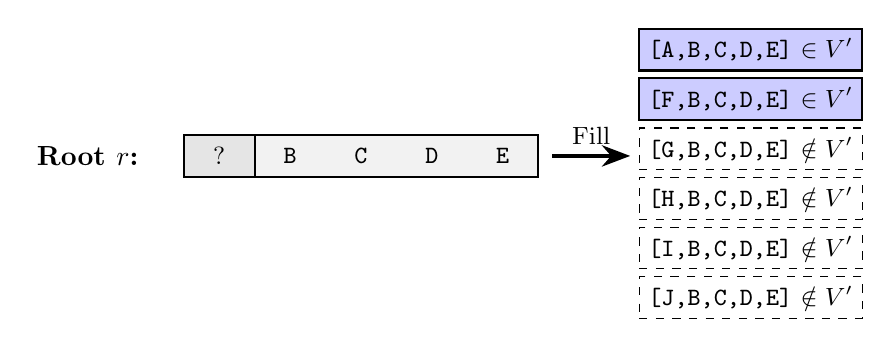
\begin{tikzpicture}[scale=0.9, font=\small, node distance=0.15cm]
			% Root definition
			\node[anchor=east, font=\bfseries] at (-0.5, 0.3) {Root $r$:};
			\draw[thick, fill=gray!20] (0,0) rectangle (1,0.6);
			\node at (0.5,0.3) {?};
			\draw[thick, fill=gray!10] (1,0) rectangle (5,0.6);
			\node at (1.5,0.3) {\texttt{B}};
			\node at (2.5,0.3) {\texttt{C}};
			\node at (3.5,0.3) {\texttt{D}};
			\node at (4.5,0.3) {\texttt{E}};

			% Expansion arrow
			\draw[->, >=Stealth, ultra thick] (5.2, 0.3) -- (6.3, 0.3) node[midway, above] {Fill};

			% Stack of vertices
			\node[draw, thick, fill=blue!20, minimum width=2.8cm, minimum height=0.5cm] (v1) at (8, 1.8) {\texttt{[A,B,C,D,E]} $\in V'$};
			\node[draw, thick, fill=blue!20, minimum width=2.8cm, minimum height=0.5cm] (v2) at (8, 1.1) {\texttt{[F,B,C,D,E]} $\in V'$};

			\node[draw, dashed, fill=white, minimum width=2.8cm, minimum height=0.5cm] (v3) at (8, 0.4) {\texttt{[G,B,C,D,E]} $\notin V'$};
			\node[draw, dashed, fill=white, minimum width=2.8cm, minimum height=0.5cm] (v4) at (8, -0.3) {\texttt{[H,B,C,D,E]} $\notin V'$};
			\node[draw, dashed, fill=white, minimum width=2.8cm, minimum height=0.5cm] (v5) at (8, -1.0) {\texttt{[I,B,C,D,E]} $\notin V'$};
			\node[draw, dashed, fill=white, minimum width=2.8cm, minimum height=0.5cm] (v6) at (8, -1.7) {\texttt{[J,B,C,D,E]} $\notin V'$};
		\end{tikzpicture}
		\caption{A single root expanding into a 1D-clique in $A(10,5)$. Vertices
		already in $V'$ form internal defect links, while the remaining empty
		slots generate the external boundary.}
		\label{fig:fill_example}
	\end{figure}
\end{example}

\begin{figure}[H]
	\centering
	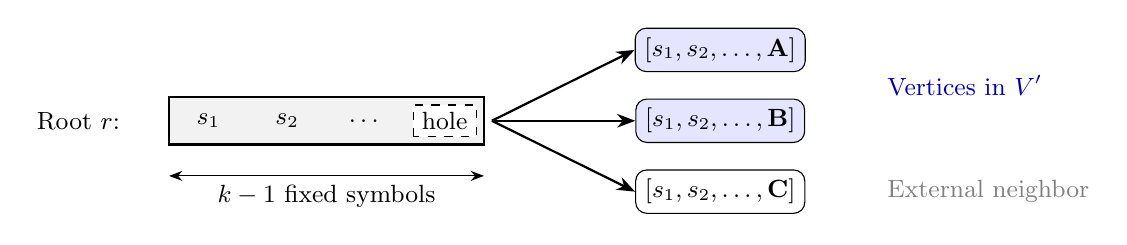
\begin{tikzpicture}[scale=1.0, font=\small]
		% Draw the "Root" (the fixed part)
		\node[anchor=east] at (-0.5,0.3) {Root $r$:};
		\draw[thick, fill=gray!10] (0,0) rectangle (4,0.6);
		\node at (0.5,0.3) {$s_1$}; \node at (1.5,0.3) {$s_2$}; \node at (2.5,0.3) {$\dots$};
		\draw[fill=white, dashed] (3.1,0.1) rectangle (3.9,0.5);
		\node at (3.5,0.3) {hole};

		% Dimension label
		\draw[<->, >=Stealth] (0,-0.4) -- (4,-0.4) node[midway, below] {$k-1$ fixed symbols};

		% Draw the "Fiber" (the extensions)
		\node (v1) at (7,1.2) [draw, rounded corners, fill=blue!10] {$[s_1, s_2, \dots, \mathbf{A}]$};
		\node (v2) at (7,0.3) [draw, rounded corners, fill=blue!10] {$[s_1, s_2, \dots, \mathbf{B}]$};
		\node (v3) at (7,-0.6) [draw, rounded corners, fill=white] {$[s_1, s_2, \dots, \mathbf{C}]$};

		\draw[->, >=Stealth, thick] (4.1,0.3) -- (v1.west);
		\draw[->, >=Stealth, thick] (4.1,0.3) -- (v2.west);
		\draw[->, >=Stealth, thick] (4.1,0.3) -- (v3.west);

		\node[anchor=west, text=blue!70!black] at (9, 0.75) {Vertices in $V'$};
		\node[anchor=west, text=gray] at (9, -0.6) {External neighbor};
	\end{tikzpicture}
	\caption{Two vertices sharing the same root (fixed $k{-}1$ symbols) are
	adjacent in $A(n,k)$. Each shared root adds one to the defect $D$ instead
	of exposing a new boundary vertex.}
	\label{fig:fiber}
\end{figure}


% ════════════════════════════════════════════════════════════════════════
\section{Algorithmic Verification}

The number of distinct connected graphs on $R$ labeled vertices grows as
$\Omega(R^{R-2})$. To check all of them, we built a symmetry-aware engine that
enumerates non-isomorphic connected subgraphs up to $R = 10$, computes their
boundary in $A(n,k)$, and identifies the minimizer. Isomorphic duplicates are
pruned via McKay's \texttt{nauty} library \cite{mckay2014practical}.

This search compares finite connected-subgraph types and computes their
boundaries over the parameter ranges recorded with the data. The defect
maximum alone does not identify boundary minimizers, because collision counts
also affect the boundary; moreover, the Hamming ball is not always optimal.
The closed-form engine evaluates the Hamming-ball candidate for arbitrary
$R$ and dimensions, but does not by itself compute the global minimum.

\begin{table}[ht]
	\centering
\caption{Hamming-ball boundary values and their verification status.}
	\label{tab:engine}
	\begin{tabular}{@{}ccccl@{}}
		\toprule
$R$ & $\Eseq(R)$ & $\Cconst(R)$ & Hamming-ball boundary & Verification                                   \\
		\midrule
		2   & 1          & 1            & $(2k-1)(n-k)-1$        & Cheng et al. \cite{cheng2022extraconnectivity} \\
		4   & 4          & 4            & $(4k-4)(n-k)-4$        & Cheng et al. \cite{cheng2022extraconnectivity} \\
		8   & 12         & 12           & $(8k-12)(n-k)-12$      & \textbf{New: value engine-verified}$^\dagger$  \\
		16  & 32         & 32           & $(16k-32)(n-k)-32$     & \textbf{New: value engine-verified}$^\dagger$  \\
		\bottomrule
	\end{tabular}
\end{table}
	\noindent $^\dagger$\small The listed value is the Hamming ball's own boundary,
	confirmed by direct construction and enumeration (Appendix~\ref{app:engine}).
	It is not asserted to be the global minimum: the full Star in $A(11,6)$ is
	a counterexample to that general claim. Finite searches establish only the
	particular graphs and volumes explicitly covered by their certificates.

\noindent \small \textit{Notably, our closed-form evaluation reveals a geometric
symmetry for perfect hypercubes ($R=2^d$): the defect mirrors the external
shadow collision constant, yielding $\Eseq(2^d) = \Cconst(2^d) = d 2^{d-1}$.}

\medskip
\noindent \textbf{Connection to Prior Literature.} Conditionally, this formula
subsumes the ad-hoc topological cases manually discovered by Cheng et al.\
\cite{cheng2022extraconnectivity} for $R \le 7$, revealing that those early
constructions were initial segments of the lexicographic Hamming Ball. Moreover,
as dimensions scale ($k,\, n{-}k \to \infty$), the constants $\Cconst(R)$ and
$\Eseq(R)$ become negligible relative to the leading $R \cdot k(n-k)$ term,
consistent with the asymptotic limits conjectured
in~\cite{cheng2022extraconnectivity}.


% ════════════════════════════════════════════════════════════════════════
\section{Failure of Geometric Compression}\label{sec:nogo}

In the Boolean hypercube $\{0,1\}^d$, shifting a vertex to use a smaller symbol
$a < b$ provably reduces (or preserves) the boundary. In arrangement graphs,
this geometric tool fundamentally fails.

\begin{theorem}[Failure of Geometric Compression]\label{thm:nogo}
There exists a subset $V' \subseteq V(A(4,2))$ such that shifting symbol $3 \to
1$ strictly \emph{increases} the external boundary from 5 to 7.
\end{theorem}

\begin{proof}
Let $V' = \{[4,3], [1,3]\}$. Before the shift, the external boundary consists of
adjacent vertices not in $V'$:
	\begin{equation*}
		\extbd(V') = \{[2,3], [4,1], [4,2], [1,2], [1,4]\} \implies \left| \extbd(V') \right| = 5
	\end{equation*}

Applying a shift $(3 \to 1)$: Vertex $[4,3]$ uses symbol 3 but not 1,
successfully shifting to $[4,1]$. However, vertex $[1,3]$ already uses 1;
shifting it would create $[1,1]$, violating permutation injectivity. Thus, it
remains unchanged. The new compressed set is $C(V') = \{[4,1], [1,3]\}$.

	The new external boundary becomes:
	\begin{equation*}
		\extbd(C(V')) = \{[2,1], [3,1], [4,2], [4,3], [2,3], [1,2], [1,4]\} \implies \left| \extbd(C(V')) \right| = 7
	\end{equation*}

Because the defect link between $[4,3]$ and $[1,3]$ was severed, the boundary
strictly increased.
\end{proof}

\begin{figure}[H]
	\centering
	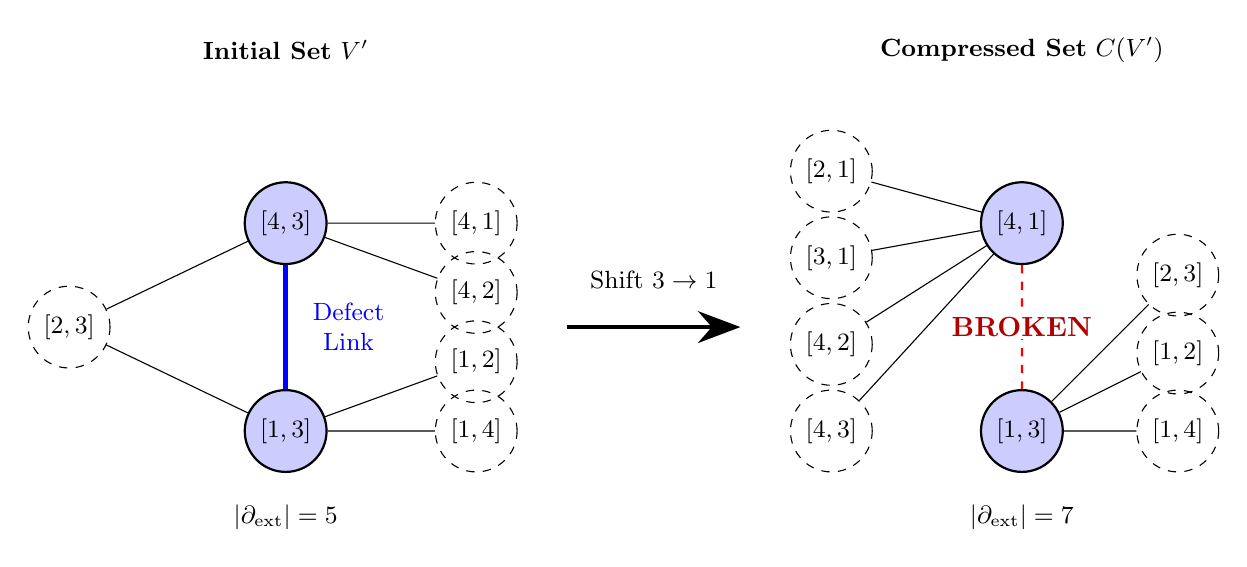
\begin{tikzpicture}[scale=1.1, node distance=2.5cm, auto, font=\small]
		% Initial Set V'
		\node at (0,3.2) {\textbf{Initial Set} $V'$};
		\node (v1) at (0,1.2) [draw, circle, fill=blue!20, thick] {$[4,3]$};
		\node (v2) at (0,-1.2) [draw, circle, fill=blue!20, thick] {$[1,3]$};
		\draw[blue, ultra thick] (v1) -- (v2) node[midway, right=0.2cm, align=center] {Defect\\Link};

		\node (n1) at (-2.5,0) [draw, circle, dashed] {$[2,3]$};
		\node (n2) at (2.2,1.2) [draw, circle, dashed] {$[4,1]$};
		\node (n3) at (2.2,0.4) [draw, circle, dashed] {$[4,2]$};
		\node (n4) at (2.2,-0.4) [draw, circle, dashed] {$[1,2]$};
		\node (n5) at (2.2,-1.2) [draw, circle, dashed] {$[1,4]$};

		\draw (v1) -- (n1); \draw (v2) -- (n1);
		\draw (v1) -- (n2); \draw (v1) -- (n3);
		\draw (v2) -- (n4); \draw (v2) -- (n5);
		\node at (0,-2.2) {$|\extbd| = 5$};

		% Transformation Arrow - CENTERED
		\draw[->, arrows={-Stealth[scale=1.5]}, ultra thick] (3.25,0) -- (5.25,0) node[midway, above=0.35cm] {Shift $3 \to 1$};

		% Compressed Set C(V')
		\node at (8.5,3.2) {\textbf{Compressed Set} $C(V')$};
		\node (u1) at (8.5,1.2) [draw, circle, fill=blue!20, thick] {$[4,1]$};
		\node (u2) at (8.5,-1.2) [draw, circle, fill=blue!20, thick] {$[1,3]$};
		% Edge is broken!
		\draw[red, dashed, thick] (u1) -- (u2);
		\node[red!70!black, font=\bfseries, fill=white, inner sep=1pt] at (8.5,0) {BROKEN};

		\node (m1) at (6.3,1.8) [draw, circle, dashed] {$[2,1]$};
		\node (m2) at (6.3,0.8) [draw, circle, dashed] {$[3,1]$};
		\node (m3) at (6.3,-0.2) [draw, circle, dashed] {$[4,2]$};
		\node (m4) at (6.3,-1.2) [draw, circle, dashed] {$[4,3]$};
		\node (m5) at (10.3,0.6) [draw, circle, dashed] {$[2,3]$};
		\node (m6) at (10.3,-0.3) [draw, circle, dashed] {$[1,2]$};
		\node (m7) at (10.3,-1.2) [draw, circle, dashed] {$[1,4]$};

		\draw (u1) -- (m1); \draw (u1) -- (m2); \draw (u1) -- (m3); \draw (u1) -- (m4);
		\draw (u2) -- (m5); \draw (u2) -- (m6); \draw (u2) -- (m7);
		\node at (8.5,-2.2) {$|\extbd| = 7$};
	\end{tikzpicture}
	\caption{Visualization of the Failure of Geometric Compression. Shifting
	symbol $3 \to 1$ in $A(4,2)$ severs a defect link because symbol 1 is
	already in use by another vertex, forcing the boundary to expand from 5 to
	7 vertices.}
	\label{fig:nogo}
\end{figure}


% ════════════════════════════════════════════════════════════════════════
\section{The Algebraic Defect Framework}\label{sec:defect}

The failure of geometric compression reveals a fundamental constraint: any
method that \emph{moves} symbols between vertices risks violating the
injectivity requirement of the arrangement graph. The algebraic defect framework
circumvents this trap entirely by abandoning vertex-level transformations in
favor of \emph{coordinate-level counting}. Rather than asking ``can we shift
vertex $v$ to reduce the boundary?'' we ask ``how many distinct projections
(roots) does $V'$ cast along each coordinate?'' This root-counting perspective
is immune to the injectivity constraint because it never attempts to reassign
symbols---it merely observes the fiber structure that the set $V'$ already
induces.

Concretely, we count global algebraic roots. The sum $U(V')$ represents the
total number of 1-dimensional ``fibers'' (coordinate-aligned cliques) that
intersect our set $V'$. Each root $r$ acts as a fixed backbone that our set
projects onto along a specific dimension.

The framework utilizes a double-counting correction. By counting the available
alphabet symbols, every unique root $r \in U_p(V')$ can be extended to exactly
$(n - k + 1)$ valid vertices in the graph. Subtracting the internal fibers
mapping into $V'$ yields the strictly external coordinate edges
$E_{\mathrm{cand}}$:
\begin{align}\label{eq:ecand}
	E_{\mathrm{cand}} & = \sum_{p=1}^k \Big( |U_p(V')| \cdot (n - k + 1) \Big) - |V'| \cdot k \nonumber                           \\
	                  & = \left(\sum_{p=1}^k |U_p(V')|\right)(n-k) - \left(|V'| \cdot k - \sum_{p=1}^k |U_p(V')|\right) \nonumber \\
	                  & = U(V') \cdot (n-k) - D(V').
\end{align}

Because external neighbors may be hit by multiple dimensions, we subtract the
\emph{Cross-Collisions} $X(V')$ to retrieve the exact boundary of unique
vertices. We formally define $X(V')$ as the sum of over-counted boundary
adjacencies:
\begin{equation}\label{eq:cross-collision}
	X(V') = \sum_{v \in \extbd(V')} (\text{deg}_{V'}(v) - 1).
\end{equation}

The exact boundary size is then:
\begin{equation}\label{eq:boundary}
	\left| \extbd(V') \right| = U(V') \cdot (n - k) - \big(X(V') + D(V')\big).
\end{equation}
The algebraic engine of this framework relies on a fundamental subadditivity
inequality for $\Eseq(\cdot)$ (Definition~2.5). While this inequality reflects
the classical inductive step in Harper's edge-isoperimetric theorem for Boolean
hypercubes \cite{harper1966optimal}, we formally mechanize it here to bound
arbitrary fiber partitions in $A(n,k)$.

\begin{lemma}[Subadditivity of A000788]\label{lem:subadditivity}
	For all $x, y \in \mathbb{N}$:
	\begin{equation}\label{eq:subadditivity}
		\Eseq(x) + \Eseq(y) + \min(x, y) \leq \Eseq(x + y).
	\end{equation}
\end{lemma}

\begin{proof}
By strong induction on $x + y$: assume \eqref{eq:subadditivity} holds for all
pairs summing to less than $x + y$. Case-split on the parity of both $x$ and $y$
(four cases) and expand via the even/odd recurrences $\Eseq(2m) = 2\, \Eseq(m) +
m$ and $\Eseq(2m+1) = \Eseq(m) + \Eseq(m+1) + m$. In each case, the recurrences
halve the arguments, reducing the inequality to the inductive hypothesis at a
strictly smaller sum. Mechanically verified in Lean~4
(\texttt{E\_add\_min\_le}).
\end{proof}

For fiber sizes $c_1,\ldots,c_m$, write $y=|U_p(V')|$. The coordinate projection
is injective on each fiber, whose roots form a subset of $U_p(V')$, so $\max_i
c_i\le y$; iterating Lemma~\ref{lem:subadditivity} while tracking this maximum
yields $\sum_i \Eseq(c_i)+R-y\le\Eseq(R)$, the multi-way bound used below.
Consequently, the Hamming Ball maximizes the defect among all connected
subgraphs.

\begin{theorem}[Defect Bound]\label{thm:defect}
	For any $R$-element subset $V' \subseteq V(A(n,k))$:
	\begin{equation}\label{eq:defect-bound}
		D(V') \leq \Eseq(R).
	\end{equation}
	Equivalently, $U(V') \geq R \cdot k - \Eseq(R)$.
\end{theorem}

\begin{proof}
By strong induction on $R$. For $R \ge 2$, choose a coordinate $p$ at which two
vertices of $V'$ disagree and partition $V'$ into fibers $\{F_\alpha\}$ by the
symbol $\alpha$ at position $p$. Each fiber is strictly smaller than $V'$, so
the inductive hypothesis gives $D(F_\alpha) \leq \Eseq(|F_\alpha|)$. The
root-disjointness structure at coordinates $q \neq p$ yields the decomposition
$D(V') \leq \sum_\alpha D(F_\alpha) + R - y$, where $y = |U_p(V')|$. Applying
the generalized partition subadditivity (iterated Lemma~\ref{lem:subadditivity})
closes the induction. Mechanically verified in Lean~4
(\texttt{sum\_unique\_roots\_lower\_bound}).
\end{proof}

Instead of relying on a dimension-independent bound on the combined waste (which
is sensitive to $n-k$ for sub-optimal topologies), the global boundary
minimality is captured by the following universal boundary inequality. Together
with the evaluation of the Hamming Ball, these two propositions form our
extremal framework.

\begin{proposition}[Universal Boundary Inequality]\label{prop:universal}
	For every $R$-element subset $V' \subseteq V(A(n,k))$:
	\begin{equation}\label{eq:universal-bound}
		\left|\extbd(V')\right| \ge \big(R \cdot k - \Eseq(R)\big) \cdot (n - k) - \Cconst(R).
	\end{equation}
\end{proposition}

\begin{proposition}[Hamming Ball Evaluation]\label{prop:hb-eval}
	The lexicographic Hamming Ball $\mathrm{HB}_R$ achieves equality:
	\begin{equation}\label{eq:hb-eval}
		X(\mathrm{HB}_R) + \Eseq(R) = \Cconst(R).
	\end{equation}
\end{proposition}

\begin{remark}
These propositions encode the extremal content of a vertex-isoperimetric
compression theorem applied to the arrangement graph fiber structure: Harper's
edge-isoperimetric theorem \cite{harper1966optimal} for the binary ($n=2$)
case, and the more general Bollob\'{a}s--Leader compression theorem for
vertex-isoperimetric inequalities on $n$-ary Hamming graphs
\cite{bollobas1991vertex} for $n > 2$. The Kruskal-Katona shadow theorem
\cite{kruskal1963number,katona1968theorem} is a related but distinct result
about uniform set systems (binary layers of the hypercube); it is not by
itself sufficient for the $n$-ary transfer required here (see the discussion
of this citation issue in the proof-sketch notes accompanying this project).
Proposition~\ref{prop:hb-eval} is
computationally verified through $R \le 160$ by constructing $\mathrm{HB}_R$ and
enumerating its boundary in $A(2R, R)$ (Appendix~\ref{app:engine}).
Proposition~\ref{prop:universal} is tested exhaustively over connected
$R$-vertex subsets for $R \le 10$ by enumerating every non-isomorphic connected
$R$-vertex subgraph via the \texttt{nauty}-based engine (Section~3), and
separately over \emph{all} (including disconnected) $R$-vertex subsets, for
$R \le 6$ across 26 parameter rows of $A(n,k)$ (up to $3.24\times10^9$ subsets
in a single row), with no counterexample found in either search. Because
both searches are bounded in $R$, this remains only partial computational
evidence; the proposition is
open, not yet proven, for general $R$. Conceptually,
Section~\ref{sec:sandwich}'s asymptotic-dominance argument explains why, once
$n-k$ is large relative to the fixed cluster size $R$, no sub-optimal topology's
savings in cross-collisions can outweigh its linear-in-$(n-k)$ penalty for
missing defect --- an argument that holds regardless of $R$, but which by itself
does not establish the exact universal bound at every finite scale; that
stronger, exact statement is exactly the content of
Proposition~\ref{prop:universal} above. A further gap, independent of these two
propositions, is the \emph{boundary-to-extraconnectivity reduction}: even with
an exact minimum-boundary theorem, one must still show that (i)~deleting the
Hamming ball's external boundary leaves every remaining component with at least
$R$~vertices, and (ii)~every minimum $(R{-}1)$-extra cut can be reduced to
isolating one connected component of exactly $R$~vertices---minimizing over
connected $R$-sets whose boundary deletion is itself a valid $(R{-}1)$-extra
cut---without increasing the cut. This reduction is not addressed in the Lean
formalization, whose capstone proves only a statement about external-neighbor
sets of $R$-element subsets. In the Lean 4 formalization, rather than declaring
these propositions as global axioms, we express this dependency by
parameterizing the public capstone theorem with the explicit
\texttt{UniversalLowerBound} hypothesis. The Hamming-ball collision evaluation
is supplied by the direct Lean proof. This cleanly isolates the classical
extremal set theory from the novel algebraic machinery
while ensuring that the compiled theorems are completely transparent, verified,
and free of raw, uninstantiated axiom commands.
\end{remark}

Combining these propositions with the boundary decomposition yields our main
result:

\begin{theorem}[Conditional Minimum-Boundary Theorem]\label{thm:main}
\textup{(Conditional on Propositions~\ref{prop:universal}
and~\ref{prop:hb-eval}; see the remark following them for their verification
status.)} For all $R \ge 2$ and $n \ge k \ge 1$:
	\begin{enumerate}
\item[\textup{(i)}] \textbf{Universal lower bound.} Every $R$-element subset $V'
\subseteq V(A(n,k))$ satisfies
		      \begin{equation}\label{eq:lower-bound}
			      \left|\extbd(V')\right| \ge \big(R \cdot k - \Eseq(R)\big) \cdot (n - k) - \Cconst(R).
		      \end{equation}
\item[\textup{(ii)}] \textbf{Achievability.} When $n - k \ge \lceil \log_2 R
\rceil$ and $k \ge \lceil \log_2 R \rceil$, the lexicographic Hamming Ball
$\mathrm{HB}_R$ achieves this bound with equality:
		      \begin{equation}\label{eq:hb-boundary}
			      \left|\extbd(\mathrm{HB}_R)\right| = \big(R \cdot k - \Eseq(R)\big) \cdot (n - k) - \Cconst(R)
		      \end{equation}
where $\Eseq(R)$ and $\Cconst(R)$ are as in Definition~2.5. Writing $d = \lceil
\log_2 R \rceil$, the correction constant admits the closed form
		      \begin{equation}\label{eq:cconst}
			      \Cconst(R) = R(d + 1) - 2^d - \Eseq(R).
		      \end{equation}
	\end{enumerate}
The embedding condition in (ii) ensures the graph is large enough to fit a
$d$-dimensional hypercube.
\end{theorem}

\begin{corollary}[Conditional Extraconnectivity Formula]\label{cor:extraconnectivity}
\textup{(Conditional on Theorem~\ref{thm:main} and the
boundary-to-extraconnectivity reduction described in the remark following
Propositions~\ref{prop:universal}--\ref{prop:hb-eval}.)} When $n - k \ge \lceil
\log_2 R \rceil$ and $k \ge \lceil \log_2 R \rceil$,
	\begin{equation}\label{eq:extraconnectivity}
		\kappa_{R-1}(A(n,k)) = \big(R \cdot k - \Eseq(R)\big) \cdot (n - k) - \Cconst(R).
	\end{equation}
\end{corollary}

\begin{remark}[Closed-form evaluation of $\Cconst$]
The summation $\sum_{i=1}^{R-1} \lceil \log_2(i+1) \rceil$ admits a closed form
by grouping indices by dimension level. For each $j \ge 1$, exactly $2^{j-1}$
indices satisfy $\lceil \log_2(i+1) \rceil = j$ (those with $2^{j-1} < i+1 \le
2^j$). Summing the complete levels $j = 1, \ldots, d-1$ via the identity
$\sum_{j=1}^{m} j \cdot 2^{j-1} = (m-1) 2^m + 1$ and adding the partial level at
$j = d$ yields
	\begin{equation}\label{eq:ceillog-sum}
		\sum_{i=1}^{R-1} \lceil \log_2(i+1) \rceil = R\,\lceil \log_2 R \rceil - 2^{\lceil \log_2 R \rceil} + 1,
	\end{equation}
	eliminating the last summation from the formula for $\Cconst(R)$.
\end{remark}

\begin{proof}
\textbf{Part~(i).} The lower bound is established directly by
Proposition~\ref{prop:universal}.

\textbf{Part~(ii).} Proposition~\ref{prop:hb-eval} shows $X(\mathrm{HB}_R) +
\Eseq(R) = \Cconst(R)$. Substituting this into the boundary decomposition
equation~\eqref{eq:boundary} for $\mathrm{HB}_R$, where $U(\mathrm{HB}_R) = R
\cdot k - \Eseq(R)$, yields
	\begin{equation}
		\left|\extbd(\mathrm{HB}_R)\right| = \big(R \cdot k - \Eseq(R)\big) \cdot (n - k) - \Cconst(R),
	\end{equation}
meaning the lexicographic Hamming Ball achieves the universal lower bound with
equality. The embedding condition ensures $A(n,k)$ has a large enough alphabet
and enough positions to realize $\mathrm{HB}_R$ as an induced subgraph.
\end{proof}

\begin{corollary}[System-Level Diagnosability]\label{cor:diagnosis}
Under the PMC and MM* models, the $g$-extra diagnosability $t_g(G)$ is derived
from the $g$-extra connectivity via $t_g(G) = \kappa_g(G) + g + 1$ when $|V(G)|
\ge 2g + 3$ \cite{cheng2023augmented}. Conditional on Theorem~\ref{thm:main},
the additional reduction from minimum $R$-set boundary to
$(R{-}1)$-extraconnectivity, and the standard size hypotheses of the relevant
PMC/MM* diagnosis theorem, the exact $(R{-}1)$-extra diagnosability of the
arrangement graph follows, extending recent diagnostic advances (e.g., adaptive
local diagnosis \cite{zhang2026three}) to arbitrary fault boundaries.
\end{corollary}

\begin{figure}[H]
	\centering
	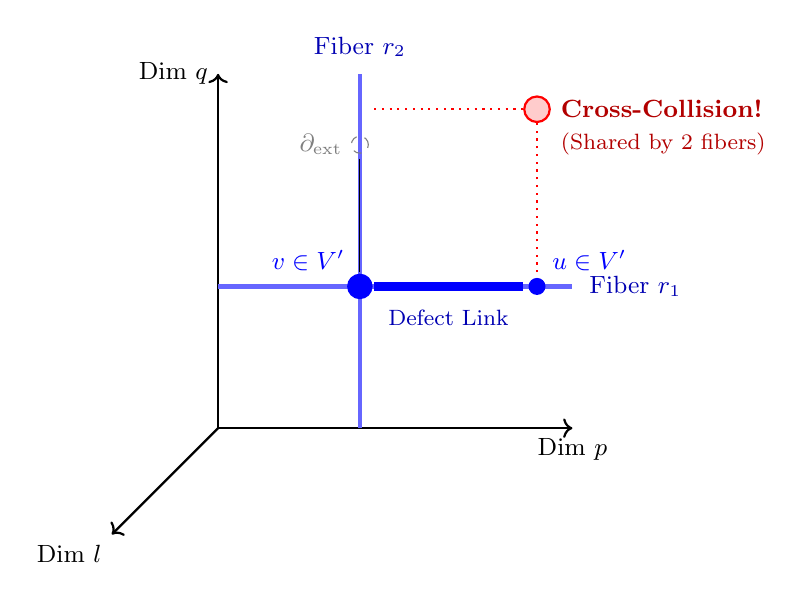
\begin{tikzpicture}[scale=0.9, font=\small]
		% Draw 3D-like axes
		\draw[->, thick] (0,0) -- (5,0) node[anchor=north] {Dim $p$};
		\draw[->, thick] (0,0) -- (0,5) node[anchor=east] {Dim $q$};
		\draw[->, thick] (0,0) -- (-1.5,-1.5) node[anchor=north east] {Dim $l$};

		% Draw "Fibers" as lines
		\draw[blue!60, ultra thick] (0,2) -- (5,2);
		\node[blue!70!black, anchor=west] at (5.1,2) {Fiber $r_1$};

		\draw[blue!60, ultra thick] (2,0) -- (2,5);
		\node[blue!70!black, anchor=south] at (2,5.1) {Fiber $r_2$};

		% Draw set V' as circles on the fibers
		\fill[blue] (2,2) circle (0.18) node[above left=0.1cm] {$v \in V'$};
		\fill[blue] (4.5,2) circle (0.12) node[above right=0.1cm] {$u \in V'$};

		% Draw internal edges (Defect)
		\draw[blue, line width=3.5pt] (2.2,2) -- (4.3,2);
		\node[blue!70!black, font=\footnotesize, anchor=north] at (3.25,1.8) {Defect Link};

		% Draw boundary vertices
		\draw[gray, dashed] (2,4) circle (0.12) node[left=0.1cm] {$\extbd$};
		\draw (2,2.2) -- (2,3.8);

		% Draw Cross-Collision
		\fill[red!20, draw=red, thick] (4.5,4.5) circle (0.18);
		\node[red!70!black, anchor=west] at (4.7,4.5) {\textbf{Cross-Collision!}};
		\node[red!70!black, font=\footnotesize, anchor=north west] at (4.7,4.3) {(Shared by 2 fibers)};

		\draw[red, dotted, thick] (2.2,4.5) -- (4.3,4.5);
		\draw[red, dotted, thick] (4.5,2.2) -- (4.5,4.3);
	\end{tikzpicture}
	\caption{The boundary decomposition
	$|\extbd(V')| = U(V') \cdot (n-k) - (X(V') + D(V'))$: defect links $D$
	shield internal vertices, while cross-collisions $X$ correct for boundary
	overlaps across coordinates.}
	\label{fig:structure}
\end{figure}

\begin{figure}[H]
	\centering
	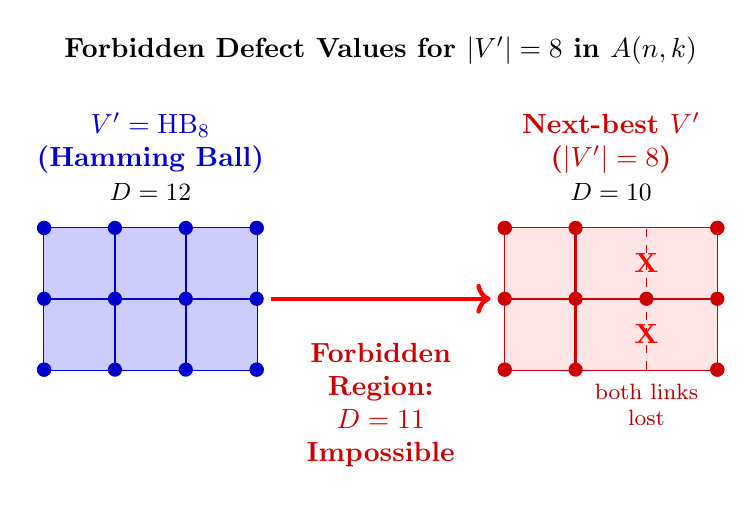
\begin{tikzpicture}[scale=0.9, font=\small]
		% Title
		\node[font=\bfseries] at (4.75, 5.5) {Forbidden Defect Values for $|V'|=8$ in $A(n,k)$};

		% Left side: Optimal subset (Hamming Ball)
		\node[align=center, font=\bfseries, text=blue!80!black] at (1.5, 4.2) {$V'=\mathrm{HB}_8$ \\ (Hamming Ball)};
		\node at (1.5, 3.5) {$D = 12$};

		\draw[thick, blue!80!black] (0,1) rectangle (3,3);
		\fill[blue!20] (0,1) rectangle (3,3);
		\foreach \x in {0,1,2,3} \foreach \y in {1,3} \fill[blue!80!black] (\x,\y) circle (0.1);
		\foreach \y in {1,2,3} \foreach \x in {0,3} \fill[blue!80!black] (\x,\y) circle (0.1);
		\draw[blue!80!black, thick] (0,2) -- (3,2);
		\draw[blue!80!black, thick] (1,1) -- (1,3);
		\draw[blue!80!black, thick] (2,1) -- (2,3);
		\fill[blue!80!black] (1,2) circle (0.1);
		\fill[blue!80!black] (2,2) circle (0.1);

		% Right side: Second Best subset
		\begin{scope}[xshift=1.5cm]
			\node[align=center, font=\bfseries, text=red!80!black] at (6.5, 4.2) {Next-best $V'$ \\ ($|V'|=8$)};
			\node at (6.5, 3.5) {$D = 10$};

			\draw[thick, red!80!black] (5,1) rectangle (8,3);
			\fill[red!10] (5,1) rectangle (8,3);
			\foreach \x in {5,6,8} \foreach \y in {1,3} \fill[red!80!black] (\x,\y) circle (0.1);
			\foreach \y in {1,2,3} \foreach \x in {5,8} \fill[red!80!black] (\x,\y) circle (0.1);
			\draw[red!80!black, thick] (5,2) -- (8,2);
			\draw[red!80!black, thick] (6,1) -- (6,3);
			\fill[red!80!black] (6,2) circle (0.1);
			\fill[red!80!black] (7,2) circle (0.1);
			\draw[red!80!black, dashed] (7,1) -- (7,3);
			\node[text=red, font=\bfseries] at (7, 2.5) {X};
			\node[text=red, font=\bfseries] at (7, 1.5) {X};
			\node[text=red!70!black, font=\footnotesize, align=center] at (7, 0.5) {both links\\lost};
		\end{scope}

		% Connecting arrow with gap label
		\draw[->, ultra thick, red] (3.2, 2) -- (6.3, 2);
		\node[align=center, font=\bfseries, text=red!80!black] at (4.75, 0.5) {Forbidden\\Region:\\$D=11$\\Impossible};
	\end{tikzpicture}
	\caption{The fracture gap at $R=8$: $\mathrm{HB}_8$ achieves $D=12$. In
	$A(n,k)$, defect links arise from root-sharing---two vertices that agree
	on all coordinates but one. Each link therefore has a ``twin'' at the same
	coordinate, so removing one vertex from a root pair destroys both links
	simultaneously. This makes $D=11$ impossible; the next achievable value is
	$D=10$.}
	\label{fig:fracture}
\end{figure}


% ════════════════════════════════════════════════════════════════════════
\section{Fixed-Topology Asymptotic Penalty}\label{sec:sandwich}

Under the per-instance hypothesis~\ref{prop:restricted_lower_bound}, together
with the independently proved evaluation~\ref{prop:hb-eval}, the Main Theorem
(Theorem~\ref{thm:main}) identifies the Hamming Ball as the conditional dense
limit. The following proposed sparse-limit comparison is refuted:

\begin{remark}[The proposed sparse-limit bound is false]
The proposed statement that every connected $R$-vertex subgraph $V'$ in
$A(n,k)$ is bounded above by the Star Graph $K_{1, R-1}$, yielding a total
correction $(X+D) = \binom{R}{2}$:
	\begin{equation}\label{eq:sparse-limit}
		\left| \extbd(V') \right| \le \big(R \cdot k - (R - 1)\big)(n - k) - \binom{R}{2}
	\end{equation}
The four-vertex path in $A(6,3)$ has external boundary $22$, while the
right-hand side of \eqref{eq:sparse-limit} is $21$, so the universal connected
version is false. A separate statement restricted to genuinely optimal
connected subgraphs is not refuted by this example, but is not proved here;
when a pairwise-distinct-symbol Star embeds, it gives the displayed value.
The inequality is retained only as a record of the abandoned heuristic and is
not used subsequently.
\end{remark}

\begin{figure}[H]
	\centering
	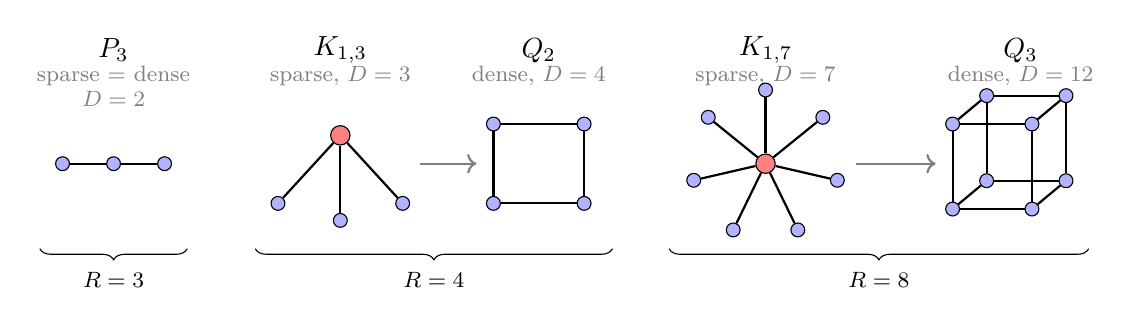
\begin{tikzpicture}[scale=0.72, font=\small,
			vertex/.style={circle, draw, fill=blue!30, inner sep=0pt, minimum size=5pt},
			hub/.style={circle, draw, fill=red!50, inner sep=0pt, minimum size=7pt}]

		% -- R=3: Path P_3 (sparse = dense) --------------------
		\node[font=\bfseries] at (0, 2.3) {$P_3$};
		\node[font=\footnotesize, text=gray] at (0, 1.85) {sparse $=$ dense};
		\node[font=\footnotesize, text=gray] at (0, 1.45) {$D=2$};

		\node[vertex] (p0) at (-0.9, 0.3) {};
		\node[vertex] (p1) at (0,    0.3) {};
		\node[vertex] (p2) at (0.9,  0.3) {};

		\draw[thick] (p0) -- (p1) -- (p2);

		% -- K_{1,3}: Star on 4 vertices -----------------------
		\node[font=\bfseries] at (4, 2.3) {$K_{1,3}$};
		\node[font=\footnotesize, text=gray] at (4, 1.85) {sparse, $D=3$};

		\node[hub]    (c1) at (4, 0.8) {};
		\node[vertex] (a1) at (2.9, -0.4) {};
		\node[vertex] (b1) at (4, -0.7) {};
		\node[vertex] (d1) at (5.1, -0.4) {};

		\draw[thick] (c1) -- (a1);
		\draw[thick] (c1) -- (b1);
		\draw[thick] (c1) -- (d1);

		% -- Q_2: Hamming Ball on 4 vertices (square) ----------
		\node[font=\bfseries] at (7.5, 2.3) {$Q_2$};
		\node[font=\footnotesize, text=gray] at (7.5, 1.85) {dense, $D=4$};

		\node[vertex] (q0) at (6.7, -0.4) {};
		\node[vertex] (q1) at (8.3, -0.4) {};
		\node[vertex] (q2) at (8.3,  1.0) {};
		\node[vertex] (q3) at (6.7,  1.0) {};

		\draw[thick] (q0) -- (q1) -- (q2) -- (q3) -- (q0);

		% Arrow between R=4 pair
		\draw[->, thick, gray] (5.4, 0.3) -- (6.4, 0.3);

		% -- K_{1,7}: Star on 8 vertices -----------------------
		\node[font=\bfseries] at (11.5, 2.3) {$K_{1,7}$};
		\node[font=\footnotesize, text=gray] at (11.5, 1.85) {sparse, $D=7$};

		\node[hub] (c2) at (11.5, 0.3) {};
		\foreach \i/\a in {1/90,2/141,3/193,4/244,5/296,6/347,7/39} {%
				\node[vertex] (s\i) at ({11.5 + 1.3*cos(\a)}, {0.3 + 1.3*sin(\a)}) {};
				\draw[thick] (c2) -- (s\i);
			}

		% -- Q_3: Hamming Ball on 8 vertices (cube) ------------
		\node[font=\bfseries] at (16, 2.3) {$Q_3$};
		\node[font=\footnotesize, text=gray] at (16, 1.85) {dense, $D=12$};

		% Front face
		\node[vertex] (f0) at (14.8, -0.5) {};
		\node[vertex] (f1) at (16.2, -0.5) {};
		\node[vertex] (f2) at (16.2,  1.0) {};
		\node[vertex] (f3) at (14.8,  1.0) {};
		% Back face (offset)
		\node[vertex] (b0) at (15.4,  0.0) {};
		\node[vertex] (b1a) at (16.8,  0.0) {};
		\node[vertex] (b2) at (16.8,  1.5) {};
		\node[vertex] (b3) at (15.4,  1.5) {};

		% Front edges
		\draw[thick] (f0) -- (f1) -- (f2) -- (f3) -- (f0);
		% Back edges
		\draw[thick] (b0) -- (b1a) -- (b2) -- (b3) -- (b0);
		% Connecting edges
		\draw[thick] (f0) -- (b0);
		\draw[thick] (f1) -- (b1a);
		\draw[thick] (f2) -- (b2);
		\draw[thick] (f3) -- (b3);

		% Arrow between R=8 pair
		\draw[->, thick, gray] (13.1, 0.3) -- (14.5, 0.3);

		% R=3 brace
		\draw[decorate, decoration={brace, mirror, amplitude=4pt}] (-1.3, -1.2) -- (1.3, -1.2)
		node[midway, below=5pt, font=\footnotesize] {$R = 3$};
		% R=4 brace
		\draw[decorate, decoration={brace, mirror, amplitude=4pt}] (2.5, -1.2) -- (8.8, -1.2)
		node[midway, below=5pt, font=\footnotesize] {$R = 4$};
		% R=8 brace
		\draw[decorate, decoration={brace, mirror, amplitude=4pt}] (9.8, -1.2) -- (17.2, -1.2)
		node[midway, below=5pt, font=\footnotesize] {$R = 8$};
	\end{tikzpicture}
	\caption{Sparse and dense limits. At $R=3$ the star graph and Hamming Ball
	coincide (both are $P_3$). At $R=4$ the gap is 1 defect link; at $R=8$ it
	widens to 5. Arrows connect the sparse limit $K_{1,R-1}$ ($D = R - 1$) to
	the dense limit $Q_d$ ($D = \Eseq(R)$).}
	\label{fig:limits}
\end{figure}

\paragraph{Structural Convergence at $R=3$.}
Our explicit bounds coincide structurally at exactly $R=3$. For the Dense Limit
(Hamming Ball), we have $\Eseq(3) = 2$ and $\Cconst(3) = 3$. For the Sparse
Limit (Star Graph), a $K_{1,2}$ structure yields defect $D = 2$,
cross-collisions $X=1$, and a total correction $(X + D) = \binom{3}{2} = 3$. The
As abstract graphs, both configurations are a three-vertex path, but their
embedded root incidences need not agree; in particular, $X$ is not determined
by the abstract graph. This records an abstract-topology coincidence, not
uniqueness of embedded extremizers.

\begin{theorem}[Fixed-Topology Asymptotic Penalty]\label{thm:penalty}
Fix a connected topology (isomorphism type) on $R$ vertices, embedded as
$V'_{\mathrm{sub}} \subseteq V(A(n,k))$, with defect shortfall $\Delta D =
\Eseq(R) - D(V'_{\mathrm{sub}}) > 0$ relative to the Hamming Ball
$V'_{\mathrm{opt}} = \mathrm{HB}_R$. Then
	\begin{equation}\label{eq:penalty-asymptotic}
		\left| \extbd(V'_{\mathrm{sub}}) \right| - \left| \extbd(V'_{\mathrm{opt}}) \right| = \Delta D \cdot (n-k) + O_R(1),
	\end{equation}
where the $O_R(1)$ term depends only on the fixed embedded configuration (not
on $n$ or $k$ once that configuration is realizable).
Consequently, for every fixed sub-optimal topology there is a threshold
$(n-k)_0$, depending only on that topology, beyond which $\left|
\extbd(V'_{\mathrm{sub}}) \right| > \left| \extbd(V'_{\mathrm{opt}}) \right|$.
\end{theorem}
To understand this mechanism, we return to the exact boundary
decomposition~\eqref{eq:boundary}:

Recall that the defect is defined as $D(V') = |V'| \cdot k - U(V')$. If a subset
$V'$ falls short of the optimal Hamming Ball defect by $\Delta D$, it must
project onto $\Delta D$ \emph{additional} unique roots to maintain its vertex
count ($U_{\mathrm{sub}} = U_{\mathrm{opt}} + \Delta D$).

Substituting this into the boundary equation yields the comparative boundary
size:
\begin{align}\label{eq:penalty-expansion}
	\left| \extbd(V'_{\mathrm{sub}}) \right| & = (U_{\mathrm{opt}} + \Delta D) \cdot (n - k) - (X_{\mathrm{sub}} + D_{\mathrm{sub}}) \nonumber                                                     \\
	                                         & = \left| \extbd(V'_{\mathrm{opt}}) \right| + \Delta D \cdot (n - k) + (X_{\mathrm{opt}} + D_{\mathrm{opt}}) - (X_{\mathrm{sub}} + D_{\mathrm{sub}})
\end{align}

This formulation isolates the asymptotic behavior. The correction term
$(X_{\mathrm{opt}} + D_{\mathrm{opt}}) - (X_{\mathrm{sub}} + D_{\mathrm{sub}})$
is a genuine constant for a fixed embedded configuration: $X$ and $D$ do not
depend on the ambient dimensions
$n, k$ once they are large enough to realize it (the same dimension-independence
exploited in the verification engine, Appendix~\ref{app:engine}). We emphasize
that we do \emph{not} claim this correction is always non-negative --- the exact
sign and magnitude vary by topology, and no dimension-independent bound of the
form $X(V')+D(V') \le f(R)$ has been established for arbitrary connected
topologies (indeed, an earlier, stronger candidate bound was refuted by an
explicit counterexample; see the discussion accompanying
Proposition~\ref{prop:restricted_lower_bound}). What is unconditionally true is only that the
correction is \emph{fixed} while $\Delta D \cdot (n-k)$ grows linearly in
$(n-k)$: for $\Delta D \ge 1$, the linear term eventually dominates any fixed
constant, however large, as $(n-k) \to \infty$. This is the precise and provable
content of the Fixed-Topology Asymptotic Penalty: it guarantees eventual, not
immediate, dominance of the Hamming Ball, with the crossover point depending on
the specific sub-optimal topology.

\subsection{Numerical Illustration}

To visualize the Fixed-Topology Asymptotic Penalty, we walk through \emph{every}
achievable defect value for connected $8$-vertex subgraphs in $A(n,k)$, where
$n$ and $k$ are the graph parameters from Definition~2.2. The Hamming Ball
($Q_3$) achieves $D = 12$; the fracture gap (Theorem~\ref{thm:fracture}) forbids
$D = 11$; and the Continuity construction (Theorem~\ref{thm:continuity}) fills
in every integer from $10$ down to $7$. The full achievable spectrum is $\{7,\,
8,\, 9,\, 10,\, 12\}$.

\begin{table}[ht]
	\centering
	\caption{Complete defect walk-through for $R=8$ in $A(n,k)$, valid for any
	$k \ge 3$.  Each row is verified by exhaustive search over all connected
	$8$-vertex subgraphs.}
	\label{tab:walkthrough_r8}
	\begin{tabular}{@{}clcl@{}}
		\toprule
		$D(V')$   & Construction                    & $U$       & Boundary                \\
		\midrule
		12        & $Q_3$ (Hamming Ball)            & $8k{-}12$ & $(8k{-}12)(n{-}k) - 12$ \\
		\emph{11} & \emph{forbidden (fracture gap)} & ---       & ---                     \\
		10        & $Q_3 - v + \text{leaf}$         & $8k{-}10$ & $(8k{-}10)(n{-}k) - 16$ \\
		9         & partial connection              & $8k{-}9$  & $(8k{-}9)(n{-}k) - 18$  \\
		8         & partial connection              & $8k{-}8$  & $(8k{-}8)(n{-}k) - 22$  \\
		7         & $K_{1,7}$ (Star Graph)          & $8k{-}7$  & $(8k{-}7)(n{-}k) - 28$  \\
		\bottomrule
	\end{tabular}
\end{table}

\noindent Each missing defect link increases $U$ by one, adding $(n{-}k)$ to the
boundary. The total correction constants ($12, 16, 18, 22, 28$) are fixed by the
graph structure and bounded by $\binom{8}{2} = 28$; as $n \to \infty$, the
boundary ranking is determined entirely by $D(V')$.

\paragraph{Convergence Near Powers of 2 ($R=7$ vs $R=8$):}
The dominance of the Hamming Ball fluctuates based on how closely $R$ fits a
perfect hypercube embedding. At $R=7$, the gap between the optimal ($D=9$) and
the 2nd best ($D=8$) is only $1(n-k)$, whereas at $R=8$, the gap jumps to
$2(n-k)$ because $D=11$ is unrealizable (Theorem~\ref{thm:fracture}). At powers
of 2, the optimal solution becomes increasingly stable relative to its nearest
competitors as the network dimensions scale.

\begin{table}[ht]
	\centering
	\caption{Defect gap between $R=7$ and $R=8$.}
	\label{tab:gap_jump}
	\begin{tabular}{@{}lccc@{}}
		\toprule
		Cluster Size $R$ & Optimal $D$ & 2nd Best $D$ & Gap ($\Delta D$) \\
		\midrule
		7 (Near-Cube)    & 9           & 8            & 1                \\
		8 (Perfect Cube) & 12          & 10           & 2                \\
		9 (Over-Cube)    & 13          & 12           & 1                \\
		\bottomrule
	\end{tabular}
\end{table}

The numerical results give fixed-topology comparisons at $n=100$.  The margin
of $464$ uses $k=4$, while the margin of $190$ uses $k=3$; they are not two
competitors in one common parameter cell.  At the common choice $k=7$, the
corresponding margins are $449$ and $182$.  These are fixed-topology
comparisons, not proofs that the Hamming Ball is the unique minimizer.

\paragraph{The Structural Inversion: Hypercubes vs.\ Arrangement Graphs.}
Comparisons with hypercube variants such as Augmented Cubes
\cite{cheng2023augmented} motivate examining Star Graphs as a competing
construction, but this paper does not establish a universal Star optimum in
either model.  The exact arrangement-graph mechanism is instead the
fixed-topology penalty: missing defect contributes a term linear in $n-k$,
while the Star produces cross-collisions that
scale quadratically as $\binom{R-1}{2}$, quickly overpowering the static penalty
and minimizing the boundary. In $A(n,k)$, however, the penalty for each missing
unit of defect is $(n-k)$ (Theorem~\ref{thm:penalty}). Because $(n-k)$ scales
with the network dimensions, it eventually dominates the static savings of a
fixed Star topology. Thus the argument establishes eventual fixed-topology
dominance only; it does not prove a permanent global inversion over all
topologies and parameter ranges.


% Corrected unconditional boundary-profile capstone; distinct from extra connectivity.
\section{An unconditional Hamming sandwich}\label{sec:hamming-sandwich}

Write $m=n-k$, and let $\Phi_{n,k}(R)$ denote the minimum external
vertex-boundary size among all $R$-element subsets of $A(n,k)$. Set
\[
 E(R)=\sum_{i=0}^{R-1}\operatorname{popcount}(i),\qquad
 C(R)=(R-1)+\sum_{i=1}^{R-1}\lceil\log_2(i+1)\rceil-E(R),
\]
and $H(R,n,k)=(Rk-E(R))m-C(R)$. When
$d=\lceil\log_2 R\rceil\leq k,m$, the Boolean Hamming ball embeds in
$A(n,k)$ and has external boundary $H(R,n,k)$; the exact evaluation is
formalized in Lean as \texttt{hamming\_ball\_eval} and
\texttt{hb\_cross\_collisions\_closed}.

For $R\geq1$, grouping the summands in $C(R)$ by binary length gives the
equivalent closed form
\begin{equation}\label{eq:cconst}
 C(R)=R\bigl(\lceil\log_2 R\rceil+1\bigr)
      -2^{\lceil\log_2 R\rceil}-E(R).
\end{equation}

The identity $\Phi_{n,k}(R)=H(R,n,k)$ does not hold in general. The embedding
conditions ensure that the Hamming-ball candidate exists; they do not make it
optimal. The full-Star certificate in
$A(11,6)$ at $R=31$ has boundary $450$, whereas $H(31,11,6)=476$.

\begin{theorem}[Unconditional boundary sandwich]\label{thm:hamming-sandwich}
For every $S\subseteq A(n,k)$ of size $R$ and $k\leq n$,
\begin{equation}\label{eq:hamming-linear-lower}
 (Rk-E(R))(n-k)\leq |N(S)|+E(R)+2(R^2-R).
\end{equation}
If the Boolean Hamming ball embeds, then
\begin{equation}\label{eq:hamming-profile-sandwich}
 \Phi_{n,k}(R)\leq H(R,n,k)
 \leq \Phi_{n,k}(R)+E(R)+2(R^2-R),
\end{equation}
and the upper comparison is witnessed by that ball. This theorem concerns
the fixed-volume vertex-boundary profile, not $g$-extra connectivity.
\end{theorem}

\begin{proof}
For each coordinate $p$, let $\partial_pS$ be the external vertices on a
$p$-line meeting $S$, and let $U(S)$ count all distinct coordinate roots
occupied by $S$. The proved root-count inequality gives
$U(S)\geq Rk-E(R)$. Counting the $m+1$ vertices on each such line and
subtracting the $Rk$ incidences from vertices of $S$ yields
\[
 |N(S)|=U(S)(m+1)-Rk-X(S),\qquad
 X(S)=\sum_p|\partial_pS|-\left|\bigcup_p\partial_pS\right|.
\]
Bonferroni's inequality bounds $X(S)$ by the sum of ordered pairwise
overlaps. The global witness-pair charging injection proves
$X(S)\leq2(R^2-R)$. Substitution gives
\[
 |N(S)|\geq(Rk-E(R))(m+1)-Rk-2(R^2-R),
\]
which is \eqref{eq:hamming-linear-lower}. The Hamming-ball witness gives
$\Phi_{n,k}(R)\leq H$. Applying the lower bound to a minimizer and using
$H\leq(Rk-E(R))m$ gives the other side of
\eqref{eq:hamming-profile-sandwich}. These counting and comparison steps are
formalized in Lean, including the global collision estimate and the capstone
profile theorem.
\end{proof}

The additive error depends on $R$ alone and is independent of $n$ and $k$.
Consequently, for fixed $R,k$ with $Rk>E(R)$, the profile has the first-order
asymptotic slope
\[
 \lim_{n\to\infty}\frac{\Phi_{n,k}(R)}{n-k}=Rk-E(R),
\]
provided the embedding condition holds (which it does for all sufficiently
large $n$ when $k\geq d$). More generally, the displayed sandwich yields a
first-order approximation whenever its explicit error is negligible relative
to $(Rk-E(R))(n-k)$. It does not classify minimizers or imply a uniform
convergence statement when $R,k$ vary with $n$.

\begin{proposition}[The zero-error claim fails]\label{prop:hamming-sandwich-sharp}
For $A(11,6)$ and $R=31$, a full radius-one Star has external boundary
$450<476=H(31,11,6)$. Thus the additive allowance in
\eqref{eq:hamming-profile-sandwich} cannot simply be deleted as a universal
claim.
\end{proposition}

This example lies at $R=km+1$, outside the small-volume regime in which a
volume-only error can be negligible relative to the leading term. It shows
that the relevant extremal geometry need not be a Hamming ball at every
volume. Determining the lower envelope of Hamming-like, Star-like, and
intermediate configurations remains open. The result above is a boundary
profile estimate only: deriving $\kappa_g$ additionally requires proving
that deleting a candidate boundary gives the required component sizes and
that every admissible extra cut is controlled by such a component. No such
reduction is asserted here.


% ════════════════════════════════════════════════════════════════════════
% ============================================================================
% gf-section.tex — drop-in section for paper.tex
% Place:  % ============================================================================
% gf-section.tex — drop-in section for paper.tex
% Place:  % ============================================================================
% gf-section.tex — drop-in section for paper.tex
% Place:  \input{gf-section}  immediately BEFORE  \section{The Fracture Gap
% and Defect Continuity}  (currently line ~702), so it follows the Asymptotic
% Penalty section whose coefficients it analyzes.
% Requires: figure at ../assets/out/delange-structure.pdf
%           (regenerate: scripts/gen_delange_figure.py)
% New bib entries: see references-additions.bib (trollope1968explicit,
% delange1975somme, allouche1992ring, allouche2003automatic,
% adamczewski2017problem, wilf2006generatingfunctionology).
% The generating-function/Mahler identities (Props ogf, mahler) and the
% closed-form/density decomposition are checked by
% scripts/verify_gf_identities.py for finitely many R (series to order 600;
% density decomposition for R < 2^16; closed forms over their scripted ranges).
% consistency check, not a proof: it does not (and cannot) establish the
% section's genuinely analytic claims — nowhere-differentiability in
% Theorem them:delange and transcendence in Corollary cor:transcend rest on
% their own arguments/citations; the supremum in Remark rem:extremal is not
% proven at all, and is presented there only as numerical evidence.
% ============================================================================

\section{Analytic Structure of the Boundary Coefficients}\label{sec:analytic}

The extraconnectivity formula~\eqref{eq:extraconnectivity} is governed by two
integer sequences: the cumulative binary weight $\Eseq(R)$ (OEIS A000788) and
the correction constant $\Cconst(R)$, linked by the closed
form~\eqref{eq:cconst}. In this section we place these coefficients in their
classical analytic context: we derive their ordinary generating functions in
the style of Wilf~\cite{wilf2006generatingfunctionology}, exhibit an exact
Mahler functional equation certifying that no linear-recurrence
(rational-generating-function) closed form for them can exist, and import the
Trollope--Delange theorem to give the exact asymptotics of the boundary
formula, including a continuous, nowhere-differentiable periodic fluctuation
that the correction density inherits. Everything in this section is an
unconditional statement about the integer sequences themselves; it does not
depend on Propositions~\ref{prop:universal} or~\ref{prop:hb-eval}. Via
Proposition~\ref{prop:hb-eval}, the difference $\Cconst(R) - \Eseq(R)$ acquires
its graph-theoretic reading as the cross-collision count $X(\mathrm{HB}_R)$,
and we use that notation for it below.

\subsection{Ordinary generating functions}

Write $s_2(i) = \mathrm{popcount}(i)$ for the binary digit sum, so
$\Eseq(R) = \sum_{i<R} s_2(i)$, and abbreviate the ceiling-log summand of
Definition~\ref{def:constants} by
$\lambda(i) = \lceil \log_2(i+1) \rceil$ (the bit length of $i$).

\begin{proposition}[Generating functions of the coefficients]\label{prop:ogf}
	As formal power series,
	\begin{align}
		\sum_{i \ge 0} s_2(i)\, x^i
		 & = \frac{1}{1-x} \sum_{j \ge 0} \frac{x^{2^j}}{1+x^{2^j}},
		\label{eq:ogf-s2}                                             \\
		\sum_{R \ge 0} \Eseq(R)\, x^R
		 & = \frac{x}{(1-x)^2} \sum_{j \ge 0} \frac{x^{2^j}}{1+x^{2^j}},
		\label{eq:ogf-E}                                              \\
		\sum_{R \ge 0} \Cconst(R)\, x^R
		 & = \frac{x^2}{(1-x)^2}
		+ \frac{x}{(1-x)^2} \sum_{j \ge 0} \frac{x^{2^{j+1}}}{1+x^{2^j}}.
		\label{eq:ogf-C}
	\end{align}
\end{proposition}

\begin{proof}
	The indicator of ``bit $j$ of $i$ is set'' is periodic in $i$ with period
	$2^{j+1}$ and pattern $0^{2^j} 1^{2^j}$; summing the geometric series over
	one period and over all periods gives
	$\sum_i [\,\text{bit } j \text{ of } i\,]\, x^i
		= x^{2^j} \frac{1-x^{2^j}}{1-x} \cdot \frac{1}{1-x^{2^{j+1}}}
		= \frac{x^{2^j}}{(1-x)(1+x^{2^j})}$.
	Summing over $j$ yields~\eqref{eq:ogf-s2} since
	$s_2 = \sum_j [\,\text{bit } j\,]$. Partial summation is multiplication by
	$x/(1-x)$: if $A(x) = \sum_i a_i x^i$ then
	$\sum_R \big(\sum_{i<R} a_i\big) x^R = \frac{x}{1-x} A(x)$, giving~\eqref{eq:ogf-E}.
	For~\eqref{eq:ogf-C}, the same period argument applied to the indicator
	$[\lambda(i) > j] = [i \ge 2^j]$ gives
	$\sum_i \lambda(i) x^i = \frac{1}{1-x}\sum_{j\ge0} x^{2^j}$, hence
	$\sum_R \big(\sum_{i<R}\lambda(i)\big) x^R = \frac{x}{(1-x)^2}\sum_j x^{2^j}$;
	combining with $\sum_{R \ge 1} (R-1)x^R = \frac{x^2}{(1-x)^2}$
	and~\eqref{eq:ogf-E} per Definition~\ref{def:constants}, the
	$\Eseq$-series cancels term-by-term against the $\lambda$-series via
	$\frac{x^{2^j}}{1} - \frac{x^{2^j}}{1+x^{2^j}} = \frac{x^{2^{j+1}}}{1+x^{2^j}}$.
\end{proof}

\subsection{A Mahler functional equation, and why no simpler closed form exists}

The radix-2 recurrences $\Eseq(2m) = 2\Eseq(m) + m$ and
$\Eseq(2m+1) = \Eseq(m) + \Eseq(m+1) + m$ that drive
Lemma~\ref{lem:subadditivity} translate, in the generating-function domain,
into a functional equation of Mahler type~--- the classical algebraic home of
divide-and-conquer sequences.

\begin{proposition}[Mahler equation]\label{prop:mahler}
	Let $S(x) = \sum_{i\ge0} s_2(i)x^i$ and $F(x) = \sum_R \Eseq(R) x^R$. Then
	\begin{equation}\label{eq:mahler}
		S(x) = (1+x)\, S(x^2) + \frac{x}{1-x^2},
		\qquad\text{equivalently}\qquad
		x\,F(x) = (1+x)^2\, F(x^2) + \frac{x^3}{(1-x)(1-x^2)} .
	\end{equation}
	In particular $S$ and $F$ are $2$-Mahler functions of order one, and
	$s_2$, $\Eseq$, and (via~\eqref{eq:cconst}) $\Cconst$ are $2$-regular
	sequences in the sense of
	Allouche--Shallit~\cite{allouche1992ring,allouche2003automatic}.
\end{proposition}

\begin{proof}
	Splitting $S$ over even and odd indices and applying
	$s_2(2m) = s_2(m)$, $s_2(2m+1) = s_2(m) + 1$ gives
	$S(x) = S(x^2) + x\,S(x^2) + x\sum_{m\ge0} x^{2m}$, which
	is~\eqref{eq:mahler}; the $F$-form follows from
	$F(x) = \frac{x}{1-x} S(x)$. Regularity of $s_2$ is the textbook example
	in~\cite{allouche1992ring}; the ring of $2$-regular sequences is closed
	under running sums (giving $\Eseq$). For $\Cconst$, write
	$d = \lceil \log_2 R \rceil$, the bit length of $R-1$ (for $R \ge 1$); it is a
	standard $2$-regular sequence~\cite{allouche1992ring}, as is
	$2^{d} = 2^{\lceil \log_2 R \rceil}$ (the round-up-to-a-power-of-$2$
	sequence), and $R$ is $2$-regular as a polynomial sequence; since the
	$2$-regular sequences form a ring (closed under both sums and products),
	$R(d{+}1) - 2^d$ is $2$-regular, and hence so is
	$\Cconst = R(d{+}1) - 2^d - \Eseq$ by~\eqref{eq:cconst}.
\end{proof}

The $2$-regular matrix representation is exactly what the characterization
engine exploits: \texttt{predict.cpp} evaluates $\Eseq(R)$ in $O(\log R)$ by
recursing on the binary expansion (Appendix~\ref{app:engine}), which is the
operational form of Proposition~\ref{prop:mahler}.

\begin{corollary}[No linear-recurrence closed form]\label{cor:transcend}
	$F(x)$ is transcendental over $\mathbb{Q}(x)$. Consequently $\Eseq(R)$
	(and hence $\Cconst(R)$) satisfies no linear recurrence with constant
	coefficients: the correction constants of
	Theorem~\ref{them:main} are not expressible by any rational generating
	function or polynomial-exponential closed form.
\end{corollary}

\begin{proof}
	We first show: no sequence of the form $a(R) = \tfrac{1}{2}R\log_2 R +
	O(R)$ is $C$-finite. Suppose $a(R) = \sum_i p_i(R)\lambda_i^R$ for
	finitely many algebraic $\lambda_i$ and polynomials $p_i$, not all zero.
	By Cauchy--Hadamard applied to the ordinary generating function of $a$,
	its radius of convergence is $1/\rho$ with $\rho = \max_i |\lambda_i|$,
	and $a(R)^{1/R} \to 1$ since $a(R) = \Theta(R\log R)$; hence $\rho = 1$,
	so every $|\lambda_i| \le 1$. Let $K \ge 0$ be the largest degree of
	$p_i$ among indices with $|\lambda_i| = 1$ (such indices exist, else
	$a(R) \to 0$), and let $h(R) = \sum_{|\lambda_i|=1} \mathrm{lead}(p_i)
	\lambda_i^R$ collect the corresponding leading coefficients; every other
	term is $o(R^K)$, so $a(R)/R^K - h(R) \to 0$. As $h$ is a nonzero finite
	sum of unit-modulus exponentials, orthogonality of distinct characters
	gives $\frac{1}{N}\sum_{R<N} |h(R)|^2 \to \sum_{|\lambda_i|=1}
	|\mathrm{lead}(p_i)|^2 > 0$, so $h$ is bounded (a finite trigonometric
	sum) but does not tend to $0$ in mean square; in particular $a(R)/R^K$
	is bounded and $\limsup_R |a(R)|/R^K > 0$. But $a(R)/R^K =
	\tfrac{1}{2}R^{1-K}\log_2 R + O(R^{1-K})$ tends to $\infty$ for $K \le 1$
	(contradicting boundedness) and to $0$ for $K \ge 2$ (contradicting
	positive limsup). No $K$ survives, so $a$ is not $C$-finite.

	Since $\Eseq(R) = \tfrac{1}{2}R\log_2 R + O(R)$ (Theorem~\ref{them:delange}
	below), $\Eseq$ is not $C$-finite by the above, so $F$ is not rational
	(a rational $F$ would make $\Eseq$ eventually satisfy a linear recurrence
	with constant coefficients, i.e.\ be $C$-finite). The identical growth
	class applies to $\Cconst$: writing $d = \lceil \log_2 R \rceil$,
	\eqref{eq:cconst} gives $\Cconst(R) = R(d{+}1) - 2^d - \Eseq(R)$, and
	since $2^{d-1} < R \le 2^d$ we have $2^d = \Theta(R)$, so
	$R(d{+}1) - 2^d = R\log_2 R + O(R)$; combined with the expansion of
	$\Eseq$ this gives $\Cconst(R) = \tfrac{1}{2}R\log_2 R + O(R)$, so
	$\Cconst$ is not $C$-finite either. A Mahler function that is algebraic
	over $\mathbb{Q}(x)$ is rational by the theorem of Adamczewski and
	Bell~\cite{adamczewski2017problem}; since $F$ satisfies~\eqref{eq:mahler}
	and is irrational, it is transcendental.
\end{proof}

\subsection{Exact asymptotics: the Trollope--Delange fluctuation}

\begin{theorem}[Trollope~\cite{trollope1968explicit};
		Delange~\cite{delange1975somme}]\label{them:delange}
	There is a continuous, nowhere-differentiable function
	$\Phi \colon \mathbb{R} \to \mathbb{R}$ of period $1$ such that for all
	$R \ge 1$,
	\begin{equation}\label{eq:delange}
		\Eseq(R) = \tfrac{1}{2} R \log_2 R + R\,\Phi(\log_2 R).
	\end{equation}
	The Fourier coefficients of $\Phi$ are known explicitly and involve the
	values of the Riemann zeta function at the points
	$2\pi i k/\log 2$ on the imaginary axis~\cite{delange1975somme}.
\end{theorem}

\begin{corollary}[Fluctuation of the correction densities]\label{cor:densities}
	Let $u = \{\log_2 R\}$ denote the fractional part and set
	$\Psi(u) = 2 - u - 2^{1-u}$. Then for all $R \ge 2$,
	\begin{align}
		\frac{\Cconst(R)}{R}
		 & = \tfrac{1}{2}\log_2 R \;+\; \Psi(u) \;-\; \Phi(\log_2 R),
		\label{eq:C-density}                                        \\
		\frac{X(\mathrm{HB}_R)}{R} \;=\; \frac{\Cconst(R)-\Eseq(R)}{R}
		 & = \Psi(u) \;-\; 2\,\Phi(\log_2 R).
		\label{eq:X-density}
	\end{align}
	In particular the cross-collision density
	$(\Cconst(R)-\Eseq(R))/R$ is a \emph{bounded}, purely oscillatory function
	of $\log_2 R$: it carries no growing term, vanishes exactly at the powers
	of two ($\Psi(0) = \Phi(d) = 0$), and is strictly positive elsewhere.
\end{corollary}

\begin{proof}
	Write $d = \lceil \log_2 R \rceil$, so for $R$ not a power of two
	$d = \log_2 R - u + 1$, and directly from the closed
	form~\eqref{eq:cconst},
	$\Cconst(R)/R = (d+1) - 2^d/R - \Eseq(R)/R
		= \log_2 R + (2 - u - 2^{1-u}) - \Eseq(R)/R$;
	substituting~\eqref{eq:delange} gives~\eqref{eq:C-density}, and
	subtracting $\Eseq(R)/R$ once more gives~\eqref{eq:X-density}. At
	$R = 2^d$ both sides agree in the limit $u \to 0^+$ and equal
	$\Cconst(2^d)/2^d - \tfrac{d}{2} = 0$, recovering
	$\Cconst(2^d) = \Eseq(2^d)$ and $X(\mathrm{HB}_{2^d}) = 0$. Boundedness
	of~\eqref{eq:X-density} follows since $\Psi$ and $\Phi$ are continuous and
	periodic; positivity away from powers of two is
	Proposition~\ref{prop:hb-eval}'s
	$X(\mathrm{HB}_R) = \Cconst(R) - \Eseq(R) \ge 0$ together with the strict
	inequality visible in the closed form.
\end{proof}

\begin{figure}[ht]
	\centering
	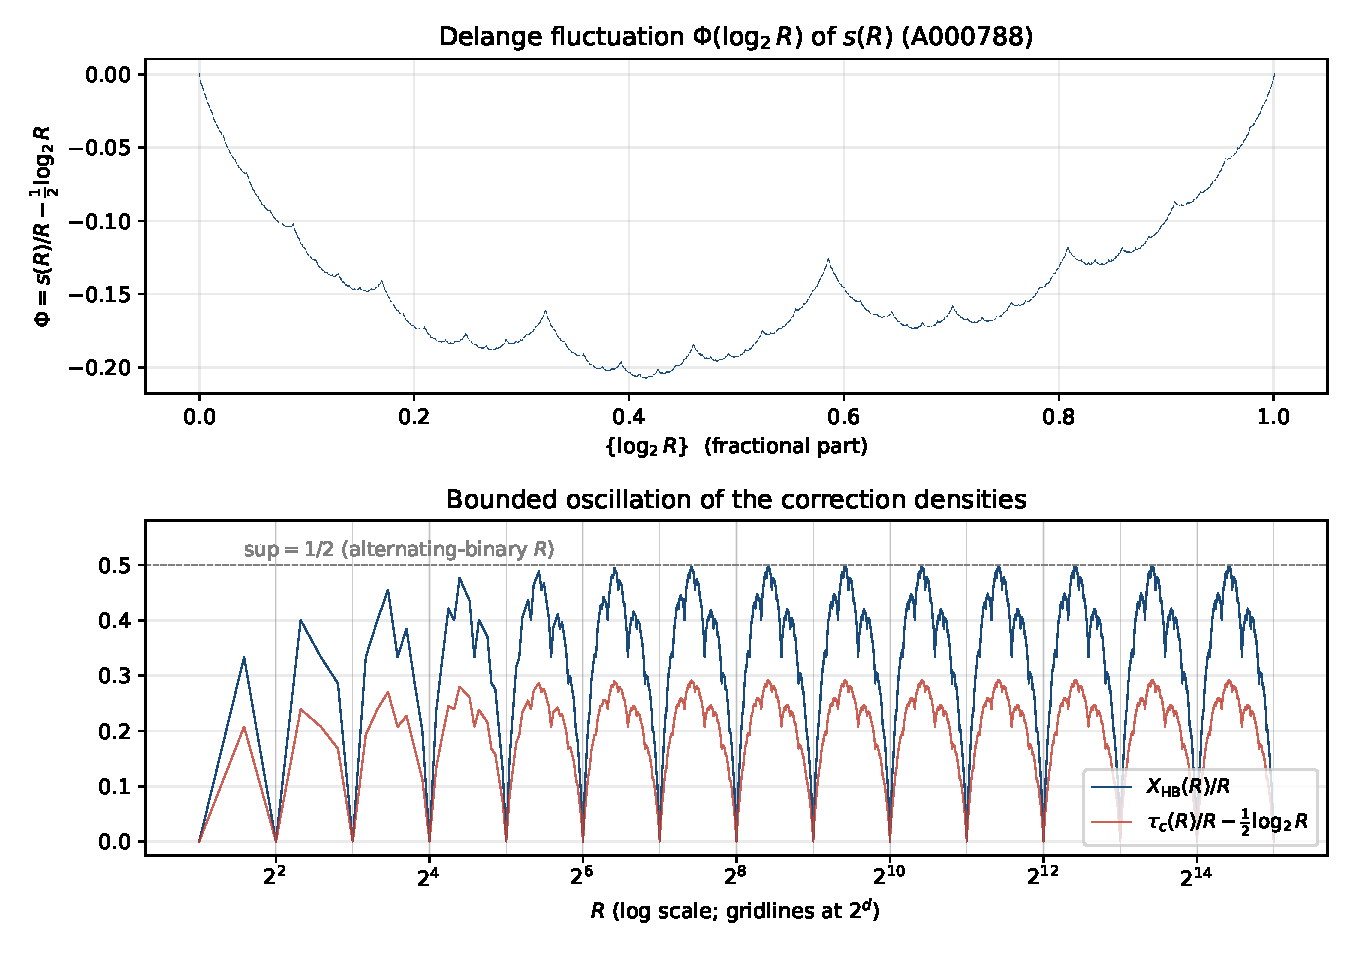
\includegraphics[width=0.92\textwidth]{../assets/out/delange-structure.pdf}
	\caption{Top: the Delange fluctuation $\Phi(\log_2 R)$
		of~\eqref{eq:delange}, computed from $\Eseq(R)$ for
		$256 \le R \le 2^{20}$ and plotted against $\{\log_2 R\}$; the
		self-similar, nowhere-differentiable profile is characteristic of
		radix-$2$ digital sums. Bottom: the centered correction density
		$\Cconst(R)/R - \tfrac{1}{2}\log_2 R$ and the cross-collision density
		$X(\mathrm{HB}_R)/R$ of Corollary~\ref{cor:densities} for
		$2 \le R \le 2^{15}$; both are bounded oscillations in $\log_2 R$,
		vanishing at every power of two (gridlines). The dashed line marks the
		empirical supremum $1/2$ of the cross-collision density, approached
		along the alternating-binary integers
		$R = \lceil 2^{d+1}/3 \rceil$ (e.g.\ $R = 43691 =
			(1010101010101011)_2$ attains $X/R > 0.49998$).}
	\label{fig:delange}
\end{figure}

\begin{remark}[Extremal densities]\label{rem:extremal}
	Numerically, $\sup_R X(\mathrm{HB}_R)/R = \tfrac{1}{2}$ for all sampled
	$R < 2^{16}$ (Figure~\ref{fig:delange}), approached along the
	alternating-binary integers $R = \lceil 2^{d+1}/3\rceil$, which are the
	classical extremizers of the Delange fluctuation; we record this as
	numerical evidence rather than a proven exact supremum, since we have
	not derived it from the Trollope--Delange expansion. The
	graph-theoretic reading is pleasing: the Hamming ball's shielding
	$4$-cycles appear, in this numerical range, to never exceed one per two
	vertices; the largest observed densities occur along the
	alternating-binary integers described above, and they disappear entirely when the ball
	closes into a full subcube.
\end{remark}

\begin{remark}[Relation to the Asymptotic Penalty]\label{rem:penalty-analogy}
	Corollary~\ref{cor:densities} quantifies exactly the $O_R(1)$ terms of
	Theorem~\ref{them:penalty}: in the boundary
	formula~\eqref{eq:extraconnectivity}, the dimension scaling contributes
	the exact linear term in $(n-k)$, while the correction density
	$\Cconst(R)/R$ splits, per~\eqref{eq:C-density}, into a logarithmic trend
	$\tfrac{1}{2}\log_2 R$ plus the bounded oscillation $\Psi(u) -
	\Phi(\log_2 R)$ that carries its entire remaining $R$-dependence.
	Readers
	familiar with analytic
	combinatorics~\cite{wilf2006generatingfunctionology} may recognize the
	division of labor: as in singularity analysis, where a dominant pole
	dictates growth and the remaining analytic part contributes bounded
	corrections, the identity of Theorem~\ref{them:penalty} separates the
	dominant $\Delta D \cdot (n-k)$ term from a topology-dependent constant
	--- though here the separation is an exact finite identity, proved
	directly in the discrete domain, rather than an asymptotic extraction.
\end{remark}
  immediately BEFORE  \section{The Fracture Gap
% and Defect Continuity}  (currently line ~702), so it follows the Asymptotic
% Penalty section whose coefficients it analyzes.
% Requires: figure at ../assets/out/delange-structure.pdf
%           (regenerate: scripts/gen_delange_figure.py)
% New bib entries: see references-additions.bib (trollope1968explicit,
% delange1975somme, allouche1992ring, allouche2003automatic,
% adamczewski2017problem, wilf2006generatingfunctionology).
% The generating-function/Mahler identities (Props ogf, mahler) and the
% closed-form/density decomposition are checked by
% scripts/verify_gf_identities.py for finitely many R (series to order 600;
% density decomposition for R < 2^16; closed forms over their scripted ranges).
% consistency check, not a proof: it does not (and cannot) establish the
% section's genuinely analytic claims — nowhere-differentiability in
% Theorem them:delange and transcendence in Corollary cor:transcend rest on
% their own arguments/citations; the supremum in Remark rem:extremal is not
% proven at all, and is presented there only as numerical evidence.
% ============================================================================

\section{Analytic Structure of the Boundary Coefficients}\label{sec:analytic}

The extraconnectivity formula~\eqref{eq:extraconnectivity} is governed by two
integer sequences: the cumulative binary weight $\Eseq(R)$ (OEIS A000788) and
the correction constant $\Cconst(R)$, linked by the closed
form~\eqref{eq:cconst}. In this section we place these coefficients in their
classical analytic context: we derive their ordinary generating functions in
the style of Wilf~\cite{wilf2006generatingfunctionology}, exhibit an exact
Mahler functional equation certifying that no linear-recurrence
(rational-generating-function) closed form for them can exist, and import the
Trollope--Delange theorem to give the exact asymptotics of the boundary
formula, including a continuous, nowhere-differentiable periodic fluctuation
that the correction density inherits. Everything in this section is an
unconditional statement about the integer sequences themselves; it does not
depend on Propositions~\ref{prop:universal} or~\ref{prop:hb-eval}. Via
Proposition~\ref{prop:hb-eval}, the difference $\Cconst(R) - \Eseq(R)$ acquires
its graph-theoretic reading as the cross-collision count $X(\mathrm{HB}_R)$,
and we use that notation for it below.

\subsection{Ordinary generating functions}

Write $s_2(i) = \mathrm{popcount}(i)$ for the binary digit sum, so
$\Eseq(R) = \sum_{i<R} s_2(i)$, and abbreviate the ceiling-log summand of
Definition~\ref{def:constants} by
$\lambda(i) = \lceil \log_2(i+1) \rceil$ (the bit length of $i$).

\begin{proposition}[Generating functions of the coefficients]\label{prop:ogf}
	As formal power series,
	\begin{align}
		\sum_{i \ge 0} s_2(i)\, x^i
		 & = \frac{1}{1-x} \sum_{j \ge 0} \frac{x^{2^j}}{1+x^{2^j}},
		\label{eq:ogf-s2}                                             \\
		\sum_{R \ge 0} \Eseq(R)\, x^R
		 & = \frac{x}{(1-x)^2} \sum_{j \ge 0} \frac{x^{2^j}}{1+x^{2^j}},
		\label{eq:ogf-E}                                              \\
		\sum_{R \ge 0} \Cconst(R)\, x^R
		 & = \frac{x^2}{(1-x)^2}
		+ \frac{x}{(1-x)^2} \sum_{j \ge 0} \frac{x^{2^{j+1}}}{1+x^{2^j}}.
		\label{eq:ogf-C}
	\end{align}
\end{proposition}

\begin{proof}
	The indicator of ``bit $j$ of $i$ is set'' is periodic in $i$ with period
	$2^{j+1}$ and pattern $0^{2^j} 1^{2^j}$; summing the geometric series over
	one period and over all periods gives
	$\sum_i [\,\text{bit } j \text{ of } i\,]\, x^i
		= x^{2^j} \frac{1-x^{2^j}}{1-x} \cdot \frac{1}{1-x^{2^{j+1}}}
		= \frac{x^{2^j}}{(1-x)(1+x^{2^j})}$.
	Summing over $j$ yields~\eqref{eq:ogf-s2} since
	$s_2 = \sum_j [\,\text{bit } j\,]$. Partial summation is multiplication by
	$x/(1-x)$: if $A(x) = \sum_i a_i x^i$ then
	$\sum_R \big(\sum_{i<R} a_i\big) x^R = \frac{x}{1-x} A(x)$, giving~\eqref{eq:ogf-E}.
	For~\eqref{eq:ogf-C}, the same period argument applied to the indicator
	$[\lambda(i) > j] = [i \ge 2^j]$ gives
	$\sum_i \lambda(i) x^i = \frac{1}{1-x}\sum_{j\ge0} x^{2^j}$, hence
	$\sum_R \big(\sum_{i<R}\lambda(i)\big) x^R = \frac{x}{(1-x)^2}\sum_j x^{2^j}$;
	combining with $\sum_{R \ge 1} (R-1)x^R = \frac{x^2}{(1-x)^2}$
	and~\eqref{eq:ogf-E} per Definition~\ref{def:constants}, the
	$\Eseq$-series cancels term-by-term against the $\lambda$-series via
	$\frac{x^{2^j}}{1} - \frac{x^{2^j}}{1+x^{2^j}} = \frac{x^{2^{j+1}}}{1+x^{2^j}}$.
\end{proof}

\subsection{A Mahler functional equation, and why no simpler closed form exists}

The radix-2 recurrences $\Eseq(2m) = 2\Eseq(m) + m$ and
$\Eseq(2m+1) = \Eseq(m) + \Eseq(m+1) + m$ that drive
Lemma~\ref{lem:subadditivity} translate, in the generating-function domain,
into a functional equation of Mahler type~--- the classical algebraic home of
divide-and-conquer sequences.

\begin{proposition}[Mahler equation]\label{prop:mahler}
	Let $S(x) = \sum_{i\ge0} s_2(i)x^i$ and $F(x) = \sum_R \Eseq(R) x^R$. Then
	\begin{equation}\label{eq:mahler}
		S(x) = (1+x)\, S(x^2) + \frac{x}{1-x^2},
		\qquad\text{equivalently}\qquad
		x\,F(x) = (1+x)^2\, F(x^2) + \frac{x^3}{(1-x)(1-x^2)} .
	\end{equation}
	In particular $S$ and $F$ are $2$-Mahler functions of order one, and
	$s_2$, $\Eseq$, and (via~\eqref{eq:cconst}) $\Cconst$ are $2$-regular
	sequences in the sense of
	Allouche--Shallit~\cite{allouche1992ring,allouche2003automatic}.
\end{proposition}

\begin{proof}
	Splitting $S$ over even and odd indices and applying
	$s_2(2m) = s_2(m)$, $s_2(2m+1) = s_2(m) + 1$ gives
	$S(x) = S(x^2) + x\,S(x^2) + x\sum_{m\ge0} x^{2m}$, which
	is~\eqref{eq:mahler}; the $F$-form follows from
	$F(x) = \frac{x}{1-x} S(x)$. Regularity of $s_2$ is the textbook example
	in~\cite{allouche1992ring}; the ring of $2$-regular sequences is closed
	under running sums (giving $\Eseq$). For $\Cconst$, write
	$d = \lceil \log_2 R \rceil$, the bit length of $R-1$ (for $R \ge 1$); it is a
	standard $2$-regular sequence~\cite{allouche1992ring}, as is
	$2^{d} = 2^{\lceil \log_2 R \rceil}$ (the round-up-to-a-power-of-$2$
	sequence), and $R$ is $2$-regular as a polynomial sequence; since the
	$2$-regular sequences form a ring (closed under both sums and products),
	$R(d{+}1) - 2^d$ is $2$-regular, and hence so is
	$\Cconst = R(d{+}1) - 2^d - \Eseq$ by~\eqref{eq:cconst}.
\end{proof}

The $2$-regular matrix representation is exactly what the characterization
engine exploits: \texttt{predict.cpp} evaluates $\Eseq(R)$ in $O(\log R)$ by
recursing on the binary expansion (Appendix~\ref{app:engine}), which is the
operational form of Proposition~\ref{prop:mahler}.

\begin{corollary}[No linear-recurrence closed form]\label{cor:transcend}
	$F(x)$ is transcendental over $\mathbb{Q}(x)$. Consequently $\Eseq(R)$
	(and hence $\Cconst(R)$) satisfies no linear recurrence with constant
	coefficients: the correction constants of
	Theorem~\ref{them:main} are not expressible by any rational generating
	function or polynomial-exponential closed form.
\end{corollary}

\begin{proof}
	We first show: no sequence of the form $a(R) = \tfrac{1}{2}R\log_2 R +
	O(R)$ is $C$-finite. Suppose $a(R) = \sum_i p_i(R)\lambda_i^R$ for
	finitely many algebraic $\lambda_i$ and polynomials $p_i$, not all zero.
	By Cauchy--Hadamard applied to the ordinary generating function of $a$,
	its radius of convergence is $1/\rho$ with $\rho = \max_i |\lambda_i|$,
	and $a(R)^{1/R} \to 1$ since $a(R) = \Theta(R\log R)$; hence $\rho = 1$,
	so every $|\lambda_i| \le 1$. Let $K \ge 0$ be the largest degree of
	$p_i$ among indices with $|\lambda_i| = 1$ (such indices exist, else
	$a(R) \to 0$), and let $h(R) = \sum_{|\lambda_i|=1} \mathrm{lead}(p_i)
	\lambda_i^R$ collect the corresponding leading coefficients; every other
	term is $o(R^K)$, so $a(R)/R^K - h(R) \to 0$. As $h$ is a nonzero finite
	sum of unit-modulus exponentials, orthogonality of distinct characters
	gives $\frac{1}{N}\sum_{R<N} |h(R)|^2 \to \sum_{|\lambda_i|=1}
	|\mathrm{lead}(p_i)|^2 > 0$, so $h$ is bounded (a finite trigonometric
	sum) but does not tend to $0$ in mean square; in particular $a(R)/R^K$
	is bounded and $\limsup_R |a(R)|/R^K > 0$. But $a(R)/R^K =
	\tfrac{1}{2}R^{1-K}\log_2 R + O(R^{1-K})$ tends to $\infty$ for $K \le 1$
	(contradicting boundedness) and to $0$ for $K \ge 2$ (contradicting
	positive limsup). No $K$ survives, so $a$ is not $C$-finite.

	Since $\Eseq(R) = \tfrac{1}{2}R\log_2 R + O(R)$ (Theorem~\ref{them:delange}
	below), $\Eseq$ is not $C$-finite by the above, so $F$ is not rational
	(a rational $F$ would make $\Eseq$ eventually satisfy a linear recurrence
	with constant coefficients, i.e.\ be $C$-finite). The identical growth
	class applies to $\Cconst$: writing $d = \lceil \log_2 R \rceil$,
	\eqref{eq:cconst} gives $\Cconst(R) = R(d{+}1) - 2^d - \Eseq(R)$, and
	since $2^{d-1} < R \le 2^d$ we have $2^d = \Theta(R)$, so
	$R(d{+}1) - 2^d = R\log_2 R + O(R)$; combined with the expansion of
	$\Eseq$ this gives $\Cconst(R) = \tfrac{1}{2}R\log_2 R + O(R)$, so
	$\Cconst$ is not $C$-finite either. A Mahler function that is algebraic
	over $\mathbb{Q}(x)$ is rational by the theorem of Adamczewski and
	Bell~\cite{adamczewski2017problem}; since $F$ satisfies~\eqref{eq:mahler}
	and is irrational, it is transcendental.
\end{proof}

\subsection{Exact asymptotics: the Trollope--Delange fluctuation}

\begin{theorem}[Trollope~\cite{trollope1968explicit};
		Delange~\cite{delange1975somme}]\label{them:delange}
	There is a continuous, nowhere-differentiable function
	$\Phi \colon \mathbb{R} \to \mathbb{R}$ of period $1$ such that for all
	$R \ge 1$,
	\begin{equation}\label{eq:delange}
		\Eseq(R) = \tfrac{1}{2} R \log_2 R + R\,\Phi(\log_2 R).
	\end{equation}
	The Fourier coefficients of $\Phi$ are known explicitly and involve the
	values of the Riemann zeta function at the points
	$2\pi i k/\log 2$ on the imaginary axis~\cite{delange1975somme}.
\end{theorem}

\begin{corollary}[Fluctuation of the correction densities]\label{cor:densities}
	Let $u = \{\log_2 R\}$ denote the fractional part and set
	$\Psi(u) = 2 - u - 2^{1-u}$. Then for all $R \ge 2$,
	\begin{align}
		\frac{\Cconst(R)}{R}
		 & = \tfrac{1}{2}\log_2 R \;+\; \Psi(u) \;-\; \Phi(\log_2 R),
		\label{eq:C-density}                                        \\
		\frac{X(\mathrm{HB}_R)}{R} \;=\; \frac{\Cconst(R)-\Eseq(R)}{R}
		 & = \Psi(u) \;-\; 2\,\Phi(\log_2 R).
		\label{eq:X-density}
	\end{align}
	In particular the cross-collision density
	$(\Cconst(R)-\Eseq(R))/R$ is a \emph{bounded}, purely oscillatory function
	of $\log_2 R$: it carries no growing term, vanishes exactly at the powers
	of two ($\Psi(0) = \Phi(d) = 0$), and is strictly positive elsewhere.
\end{corollary}

\begin{proof}
	Write $d = \lceil \log_2 R \rceil$, so for $R$ not a power of two
	$d = \log_2 R - u + 1$, and directly from the closed
	form~\eqref{eq:cconst},
	$\Cconst(R)/R = (d+1) - 2^d/R - \Eseq(R)/R
		= \log_2 R + (2 - u - 2^{1-u}) - \Eseq(R)/R$;
	substituting~\eqref{eq:delange} gives~\eqref{eq:C-density}, and
	subtracting $\Eseq(R)/R$ once more gives~\eqref{eq:X-density}. At
	$R = 2^d$ both sides agree in the limit $u \to 0^+$ and equal
	$\Cconst(2^d)/2^d - \tfrac{d}{2} = 0$, recovering
	$\Cconst(2^d) = \Eseq(2^d)$ and $X(\mathrm{HB}_{2^d}) = 0$. Boundedness
	of~\eqref{eq:X-density} follows since $\Psi$ and $\Phi$ are continuous and
	periodic; positivity away from powers of two is
	Proposition~\ref{prop:hb-eval}'s
	$X(\mathrm{HB}_R) = \Cconst(R) - \Eseq(R) \ge 0$ together with the strict
	inequality visible in the closed form.
\end{proof}

\begin{figure}[ht]
	\centering
	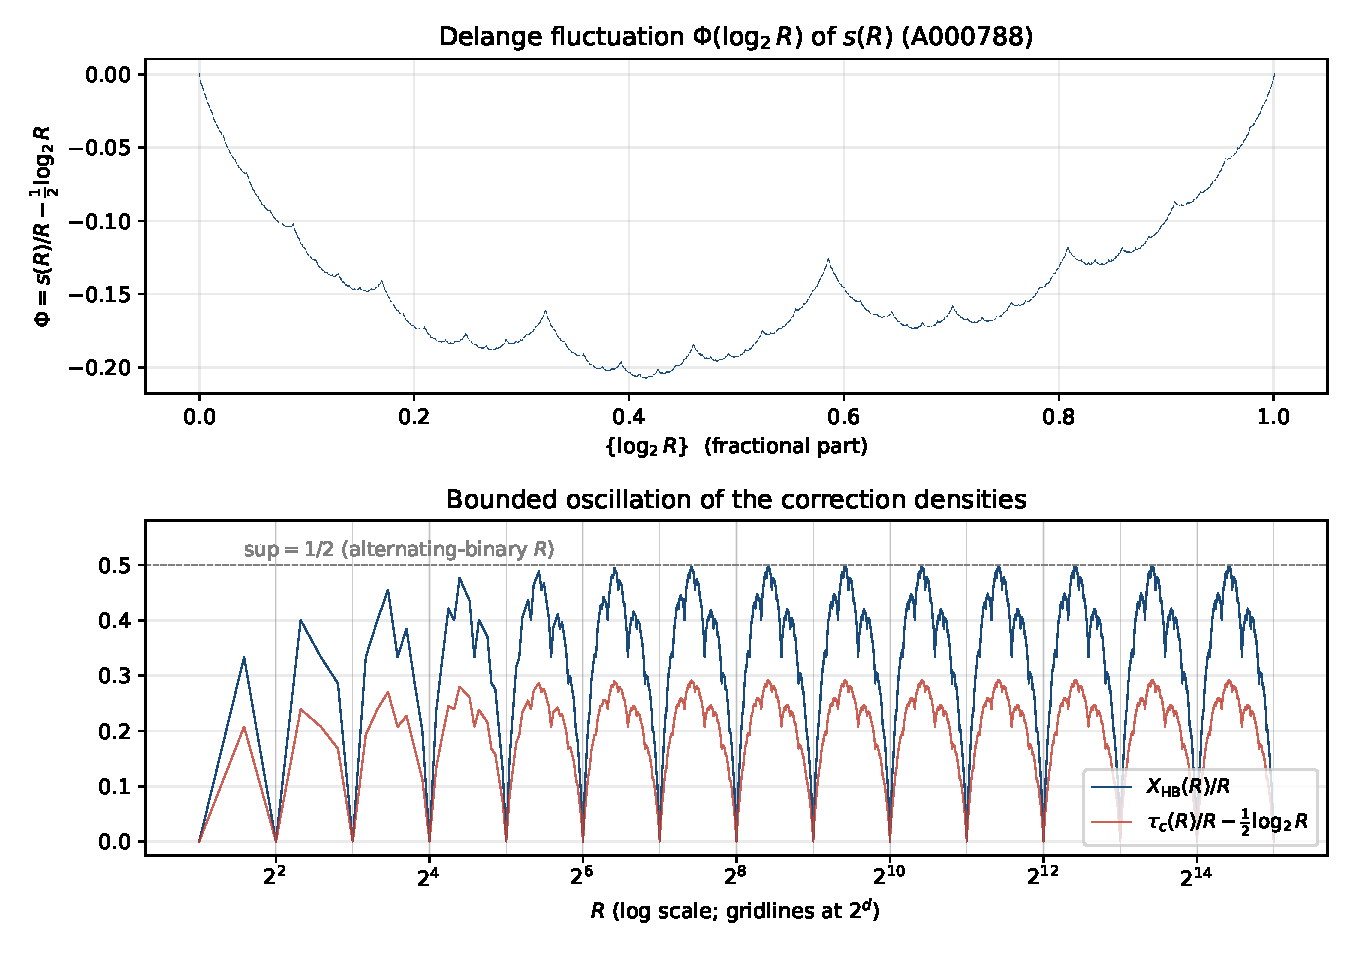
\includegraphics[width=0.92\textwidth]{../assets/out/delange-structure.pdf}
	\caption{Top: the Delange fluctuation $\Phi(\log_2 R)$
		of~\eqref{eq:delange}, computed from $\Eseq(R)$ for
		$256 \le R \le 2^{20}$ and plotted against $\{\log_2 R\}$; the
		self-similar, nowhere-differentiable profile is characteristic of
		radix-$2$ digital sums. Bottom: the centered correction density
		$\Cconst(R)/R - \tfrac{1}{2}\log_2 R$ and the cross-collision density
		$X(\mathrm{HB}_R)/R$ of Corollary~\ref{cor:densities} for
		$2 \le R \le 2^{15}$; both are bounded oscillations in $\log_2 R$,
		vanishing at every power of two (gridlines). The dashed line marks the
		empirical supremum $1/2$ of the cross-collision density, approached
		along the alternating-binary integers
		$R = \lceil 2^{d+1}/3 \rceil$ (e.g.\ $R = 43691 =
			(1010101010101011)_2$ attains $X/R > 0.49998$).}
	\label{fig:delange}
\end{figure}

\begin{remark}[Extremal densities]\label{rem:extremal}
	Numerically, $\sup_R X(\mathrm{HB}_R)/R = \tfrac{1}{2}$ for all sampled
	$R < 2^{16}$ (Figure~\ref{fig:delange}), approached along the
	alternating-binary integers $R = \lceil 2^{d+1}/3\rceil$, which are the
	classical extremizers of the Delange fluctuation; we record this as
	numerical evidence rather than a proven exact supremum, since we have
	not derived it from the Trollope--Delange expansion. The
	graph-theoretic reading is pleasing: the Hamming ball's shielding
	$4$-cycles appear, in this numerical range, to never exceed one per two
	vertices; the largest observed densities occur along the
	alternating-binary integers described above, and they disappear entirely when the ball
	closes into a full subcube.
\end{remark}

\begin{remark}[Relation to the Asymptotic Penalty]\label{rem:penalty-analogy}
	Corollary~\ref{cor:densities} quantifies exactly the $O_R(1)$ terms of
	Theorem~\ref{them:penalty}: in the boundary
	formula~\eqref{eq:extraconnectivity}, the dimension scaling contributes
	the exact linear term in $(n-k)$, while the correction density
	$\Cconst(R)/R$ splits, per~\eqref{eq:C-density}, into a logarithmic trend
	$\tfrac{1}{2}\log_2 R$ plus the bounded oscillation $\Psi(u) -
	\Phi(\log_2 R)$ that carries its entire remaining $R$-dependence.
	Readers
	familiar with analytic
	combinatorics~\cite{wilf2006generatingfunctionology} may recognize the
	division of labor: as in singularity analysis, where a dominant pole
	dictates growth and the remaining analytic part contributes bounded
	corrections, the identity of Theorem~\ref{them:penalty} separates the
	dominant $\Delta D \cdot (n-k)$ term from a topology-dependent constant
	--- though here the separation is an exact finite identity, proved
	directly in the discrete domain, rather than an asymptotic extraction.
\end{remark}
  immediately BEFORE  \section{The Fracture Gap
% and Defect Continuity}  (currently line ~702), so it follows the Asymptotic
% Penalty section whose coefficients it analyzes.
% Requires: figure at ../assets/out/delange-structure.pdf
%           (regenerate: scripts/gen_delange_figure.py)
% New bib entries: see references-additions.bib (trollope1968explicit,
% delange1975somme, allouche1992ring, allouche2003automatic,
% adamczewski2017problem, wilf2006generatingfunctionology).
% The generating-function/Mahler identities (Props ogf, mahler) and the
% closed-form/density decomposition are checked by
% scripts/verify_gf_identities.py for finitely many R (series to order 600;
% density decomposition for R < 2^16; closed forms over their scripted ranges).
% consistency check, not a proof: it does not (and cannot) establish the
% section's genuinely analytic claims — nowhere-differentiability in
% Theorem them:delange and transcendence in Corollary cor:transcend rest on
% their own arguments/citations; the supremum in Remark rem:extremal is not
% proven at all, and is presented there only as numerical evidence.
% ============================================================================

\section{Analytic Structure of the Boundary Coefficients}\label{sec:analytic}

The extraconnectivity formula~\eqref{eq:extraconnectivity} is governed by two
integer sequences: the cumulative binary weight $\Eseq(R)$ (OEIS A000788) and
the correction constant $\Cconst(R)$, linked by the closed
form~\eqref{eq:cconst}. In this section we place these coefficients in their
classical analytic context: we derive their ordinary generating functions in
the style of Wilf~\cite{wilf2006generatingfunctionology}, exhibit an exact
Mahler functional equation certifying that no linear-recurrence
(rational-generating-function) closed form for them can exist, and import the
Trollope--Delange theorem to give the exact asymptotics of the boundary
formula, including a continuous, nowhere-differentiable periodic fluctuation
that the correction density inherits. Everything in this section is an
unconditional statement about the integer sequences themselves; it does not
depend on Propositions~\ref{prop:universal} or~\ref{prop:hb-eval}. Via
Proposition~\ref{prop:hb-eval}, the difference $\Cconst(R) - \Eseq(R)$ acquires
its graph-theoretic reading as the cross-collision count $X(\mathrm{HB}_R)$,
and we use that notation for it below.

\subsection{Ordinary generating functions}

Write $s_2(i) = \mathrm{popcount}(i)$ for the binary digit sum, so
$\Eseq(R) = \sum_{i<R} s_2(i)$, and abbreviate the ceiling-log summand of
Definition~\ref{def:constants} by
$\lambda(i) = \lceil \log_2(i+1) \rceil$ (the bit length of $i$).

\begin{proposition}[Generating functions of the coefficients]\label{prop:ogf}
	As formal power series,
	\begin{align}
		\sum_{i \ge 0} s_2(i)\, x^i
		 & = \frac{1}{1-x} \sum_{j \ge 0} \frac{x^{2^j}}{1+x^{2^j}},
		\label{eq:ogf-s2}                                             \\
		\sum_{R \ge 0} \Eseq(R)\, x^R
		 & = \frac{x}{(1-x)^2} \sum_{j \ge 0} \frac{x^{2^j}}{1+x^{2^j}},
		\label{eq:ogf-E}                                              \\
		\sum_{R \ge 0} \Cconst(R)\, x^R
		 & = \frac{x^2}{(1-x)^2}
		+ \frac{x}{(1-x)^2} \sum_{j \ge 0} \frac{x^{2^{j+1}}}{1+x^{2^j}}.
		\label{eq:ogf-C}
	\end{align}
\end{proposition}

\begin{proof}
	The indicator of ``bit $j$ of $i$ is set'' is periodic in $i$ with period
	$2^{j+1}$ and pattern $0^{2^j} 1^{2^j}$; summing the geometric series over
	one period and over all periods gives
	$\sum_i [\,\text{bit } j \text{ of } i\,]\, x^i
		= x^{2^j} \frac{1-x^{2^j}}{1-x} \cdot \frac{1}{1-x^{2^{j+1}}}
		= \frac{x^{2^j}}{(1-x)(1+x^{2^j})}$.
	Summing over $j$ yields~\eqref{eq:ogf-s2} since
	$s_2 = \sum_j [\,\text{bit } j\,]$. Partial summation is multiplication by
	$x/(1-x)$: if $A(x) = \sum_i a_i x^i$ then
	$\sum_R \big(\sum_{i<R} a_i\big) x^R = \frac{x}{1-x} A(x)$, giving~\eqref{eq:ogf-E}.
	For~\eqref{eq:ogf-C}, the same period argument applied to the indicator
	$[\lambda(i) > j] = [i \ge 2^j]$ gives
	$\sum_i \lambda(i) x^i = \frac{1}{1-x}\sum_{j\ge0} x^{2^j}$, hence
	$\sum_R \big(\sum_{i<R}\lambda(i)\big) x^R = \frac{x}{(1-x)^2}\sum_j x^{2^j}$;
	combining with $\sum_{R \ge 1} (R-1)x^R = \frac{x^2}{(1-x)^2}$
	and~\eqref{eq:ogf-E} per Definition~\ref{def:constants}, the
	$\Eseq$-series cancels term-by-term against the $\lambda$-series via
	$\frac{x^{2^j}}{1} - \frac{x^{2^j}}{1+x^{2^j}} = \frac{x^{2^{j+1}}}{1+x^{2^j}}$.
\end{proof}

\subsection{A Mahler functional equation, and why no simpler closed form exists}

The radix-2 recurrences $\Eseq(2m) = 2\Eseq(m) + m$ and
$\Eseq(2m+1) = \Eseq(m) + \Eseq(m+1) + m$ that drive
Lemma~\ref{lem:subadditivity} translate, in the generating-function domain,
into a functional equation of Mahler type~--- the classical algebraic home of
divide-and-conquer sequences.

\begin{proposition}[Mahler equation]\label{prop:mahler}
	Let $S(x) = \sum_{i\ge0} s_2(i)x^i$ and $F(x) = \sum_R \Eseq(R) x^R$. Then
	\begin{equation}\label{eq:mahler}
		S(x) = (1+x)\, S(x^2) + \frac{x}{1-x^2},
		\qquad\text{equivalently}\qquad
		x\,F(x) = (1+x)^2\, F(x^2) + \frac{x^3}{(1-x)(1-x^2)} .
	\end{equation}
	In particular $S$ and $F$ are $2$-Mahler functions of order one, and
	$s_2$, $\Eseq$, and (via~\eqref{eq:cconst}) $\Cconst$ are $2$-regular
	sequences in the sense of
	Allouche--Shallit~\cite{allouche1992ring,allouche2003automatic}.
\end{proposition}

\begin{proof}
	Splitting $S$ over even and odd indices and applying
	$s_2(2m) = s_2(m)$, $s_2(2m+1) = s_2(m) + 1$ gives
	$S(x) = S(x^2) + x\,S(x^2) + x\sum_{m\ge0} x^{2m}$, which
	is~\eqref{eq:mahler}; the $F$-form follows from
	$F(x) = \frac{x}{1-x} S(x)$. Regularity of $s_2$ is the textbook example
	in~\cite{allouche1992ring}; the ring of $2$-regular sequences is closed
	under running sums (giving $\Eseq$). For $\Cconst$, write
	$d = \lceil \log_2 R \rceil$, the bit length of $R-1$ (for $R \ge 1$); it is a
	standard $2$-regular sequence~\cite{allouche1992ring}, as is
	$2^{d} = 2^{\lceil \log_2 R \rceil}$ (the round-up-to-a-power-of-$2$
	sequence), and $R$ is $2$-regular as a polynomial sequence; since the
	$2$-regular sequences form a ring (closed under both sums and products),
	$R(d{+}1) - 2^d$ is $2$-regular, and hence so is
	$\Cconst = R(d{+}1) - 2^d - \Eseq$ by~\eqref{eq:cconst}.
\end{proof}

The $2$-regular matrix representation is exactly what the characterization
engine exploits: \texttt{predict.cpp} evaluates $\Eseq(R)$ in $O(\log R)$ by
recursing on the binary expansion (Appendix~\ref{app:engine}), which is the
operational form of Proposition~\ref{prop:mahler}.

\begin{corollary}[No linear-recurrence closed form]\label{cor:transcend}
	$F(x)$ is transcendental over $\mathbb{Q}(x)$. Consequently $\Eseq(R)$
	(and hence $\Cconst(R)$) satisfies no linear recurrence with constant
	coefficients: the correction constants of
	Theorem~\ref{them:main} are not expressible by any rational generating
	function or polynomial-exponential closed form.
\end{corollary}

\begin{proof}
	We first show: no sequence of the form $a(R) = \tfrac{1}{2}R\log_2 R +
	O(R)$ is $C$-finite. Suppose $a(R) = \sum_i p_i(R)\lambda_i^R$ for
	finitely many algebraic $\lambda_i$ and polynomials $p_i$, not all zero.
	By Cauchy--Hadamard applied to the ordinary generating function of $a$,
	its radius of convergence is $1/\rho$ with $\rho = \max_i |\lambda_i|$,
	and $a(R)^{1/R} \to 1$ since $a(R) = \Theta(R\log R)$; hence $\rho = 1$,
	so every $|\lambda_i| \le 1$. Let $K \ge 0$ be the largest degree of
	$p_i$ among indices with $|\lambda_i| = 1$ (such indices exist, else
	$a(R) \to 0$), and let $h(R) = \sum_{|\lambda_i|=1} \mathrm{lead}(p_i)
	\lambda_i^R$ collect the corresponding leading coefficients; every other
	term is $o(R^K)$, so $a(R)/R^K - h(R) \to 0$. As $h$ is a nonzero finite
	sum of unit-modulus exponentials, orthogonality of distinct characters
	gives $\frac{1}{N}\sum_{R<N} |h(R)|^2 \to \sum_{|\lambda_i|=1}
	|\mathrm{lead}(p_i)|^2 > 0$, so $h$ is bounded (a finite trigonometric
	sum) but does not tend to $0$ in mean square; in particular $a(R)/R^K$
	is bounded and $\limsup_R |a(R)|/R^K > 0$. But $a(R)/R^K =
	\tfrac{1}{2}R^{1-K}\log_2 R + O(R^{1-K})$ tends to $\infty$ for $K \le 1$
	(contradicting boundedness) and to $0$ for $K \ge 2$ (contradicting
	positive limsup). No $K$ survives, so $a$ is not $C$-finite.

	Since $\Eseq(R) = \tfrac{1}{2}R\log_2 R + O(R)$ (Theorem~\ref{them:delange}
	below), $\Eseq$ is not $C$-finite by the above, so $F$ is not rational
	(a rational $F$ would make $\Eseq$ eventually satisfy a linear recurrence
	with constant coefficients, i.e.\ be $C$-finite). The identical growth
	class applies to $\Cconst$: writing $d = \lceil \log_2 R \rceil$,
	\eqref{eq:cconst} gives $\Cconst(R) = R(d{+}1) - 2^d - \Eseq(R)$, and
	since $2^{d-1} < R \le 2^d$ we have $2^d = \Theta(R)$, so
	$R(d{+}1) - 2^d = R\log_2 R + O(R)$; combined with the expansion of
	$\Eseq$ this gives $\Cconst(R) = \tfrac{1}{2}R\log_2 R + O(R)$, so
	$\Cconst$ is not $C$-finite either. A Mahler function that is algebraic
	over $\mathbb{Q}(x)$ is rational by the theorem of Adamczewski and
	Bell~\cite{adamczewski2017problem}; since $F$ satisfies~\eqref{eq:mahler}
	and is irrational, it is transcendental.
\end{proof}

\subsection{Exact asymptotics: the Trollope--Delange fluctuation}

\begin{theorem}[Trollope~\cite{trollope1968explicit};
		Delange~\cite{delange1975somme}]\label{them:delange}
	There is a continuous, nowhere-differentiable function
	$\Phi \colon \mathbb{R} \to \mathbb{R}$ of period $1$ such that for all
	$R \ge 1$,
	\begin{equation}\label{eq:delange}
		\Eseq(R) = \tfrac{1}{2} R \log_2 R + R\,\Phi(\log_2 R).
	\end{equation}
	The Fourier coefficients of $\Phi$ are known explicitly and involve the
	values of the Riemann zeta function at the points
	$2\pi i k/\log 2$ on the imaginary axis~\cite{delange1975somme}.
\end{theorem}

\begin{corollary}[Fluctuation of the correction densities]\label{cor:densities}
	Let $u = \{\log_2 R\}$ denote the fractional part and set
	$\Psi(u) = 2 - u - 2^{1-u}$. Then for all $R \ge 2$,
	\begin{align}
		\frac{\Cconst(R)}{R}
		 & = \tfrac{1}{2}\log_2 R \;+\; \Psi(u) \;-\; \Phi(\log_2 R),
		\label{eq:C-density}                                        \\
		\frac{X(\mathrm{HB}_R)}{R} \;=\; \frac{\Cconst(R)-\Eseq(R)}{R}
		 & = \Psi(u) \;-\; 2\,\Phi(\log_2 R).
		\label{eq:X-density}
	\end{align}
	In particular the cross-collision density
	$(\Cconst(R)-\Eseq(R))/R$ is a \emph{bounded}, purely oscillatory function
	of $\log_2 R$: it carries no growing term, vanishes exactly at the powers
	of two ($\Psi(0) = \Phi(d) = 0$), and is strictly positive elsewhere.
\end{corollary}

\begin{proof}
	Write $d = \lceil \log_2 R \rceil$, so for $R$ not a power of two
	$d = \log_2 R - u + 1$, and directly from the closed
	form~\eqref{eq:cconst},
	$\Cconst(R)/R = (d+1) - 2^d/R - \Eseq(R)/R
		= \log_2 R + (2 - u - 2^{1-u}) - \Eseq(R)/R$;
	substituting~\eqref{eq:delange} gives~\eqref{eq:C-density}, and
	subtracting $\Eseq(R)/R$ once more gives~\eqref{eq:X-density}. At
	$R = 2^d$ both sides agree in the limit $u \to 0^+$ and equal
	$\Cconst(2^d)/2^d - \tfrac{d}{2} = 0$, recovering
	$\Cconst(2^d) = \Eseq(2^d)$ and $X(\mathrm{HB}_{2^d}) = 0$. Boundedness
	of~\eqref{eq:X-density} follows since $\Psi$ and $\Phi$ are continuous and
	periodic; positivity away from powers of two is
	Proposition~\ref{prop:hb-eval}'s
	$X(\mathrm{HB}_R) = \Cconst(R) - \Eseq(R) \ge 0$ together with the strict
	inequality visible in the closed form.
\end{proof}

\begin{figure}[ht]
	\centering
	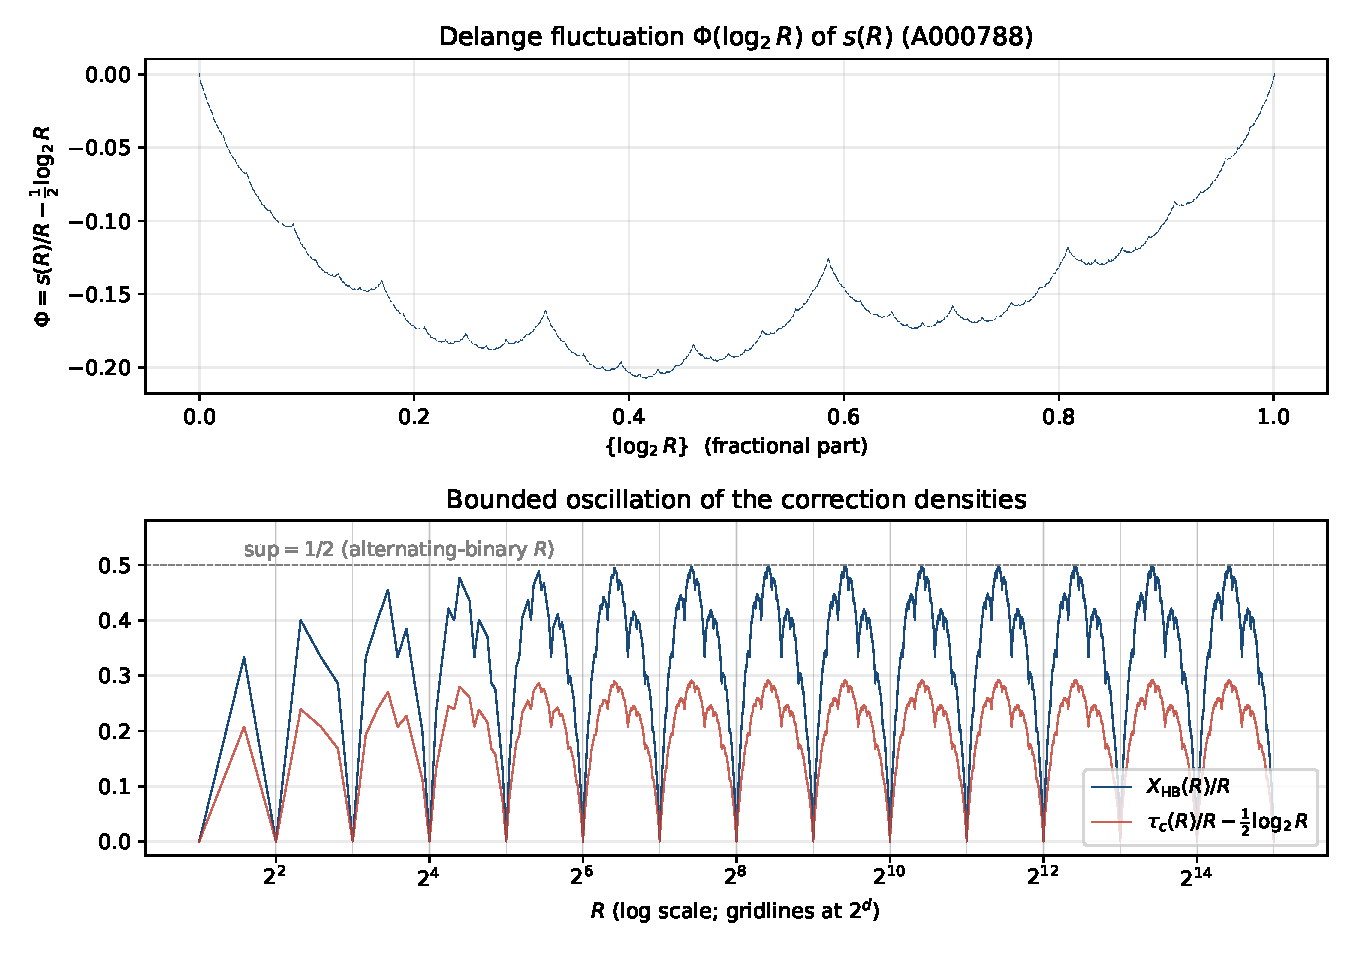
\includegraphics[width=0.92\textwidth]{../assets/out/delange-structure.pdf}
	\caption{Top: the Delange fluctuation $\Phi(\log_2 R)$
		of~\eqref{eq:delange}, computed from $\Eseq(R)$ for
		$256 \le R \le 2^{20}$ and plotted against $\{\log_2 R\}$; the
		self-similar, nowhere-differentiable profile is characteristic of
		radix-$2$ digital sums. Bottom: the centered correction density
		$\Cconst(R)/R - \tfrac{1}{2}\log_2 R$ and the cross-collision density
		$X(\mathrm{HB}_R)/R$ of Corollary~\ref{cor:densities} for
		$2 \le R \le 2^{15}$; both are bounded oscillations in $\log_2 R$,
		vanishing at every power of two (gridlines). The dashed line marks the
		empirical supremum $1/2$ of the cross-collision density, approached
		along the alternating-binary integers
		$R = \lceil 2^{d+1}/3 \rceil$ (e.g.\ $R = 43691 =
			(1010101010101011)_2$ attains $X/R > 0.49998$).}
	\label{fig:delange}
\end{figure}

\begin{remark}[Extremal densities]\label{rem:extremal}
	Numerically, $\sup_R X(\mathrm{HB}_R)/R = \tfrac{1}{2}$ for all sampled
	$R < 2^{16}$ (Figure~\ref{fig:delange}), approached along the
	alternating-binary integers $R = \lceil 2^{d+1}/3\rceil$, which are the
	classical extremizers of the Delange fluctuation; we record this as
	numerical evidence rather than a proven exact supremum, since we have
	not derived it from the Trollope--Delange expansion. The
	graph-theoretic reading is pleasing: the Hamming ball's shielding
	$4$-cycles appear, in this numerical range, to never exceed one per two
	vertices; the largest observed densities occur along the
	alternating-binary integers described above, and they disappear entirely when the ball
	closes into a full subcube.
\end{remark}

\begin{remark}[Relation to the Asymptotic Penalty]\label{rem:penalty-analogy}
	Corollary~\ref{cor:densities} quantifies exactly the $O_R(1)$ terms of
	Theorem~\ref{them:penalty}: in the boundary
	formula~\eqref{eq:extraconnectivity}, the dimension scaling contributes
	the exact linear term in $(n-k)$, while the correction density
	$\Cconst(R)/R$ splits, per~\eqref{eq:C-density}, into a logarithmic trend
	$\tfrac{1}{2}\log_2 R$ plus the bounded oscillation $\Psi(u) -
	\Phi(\log_2 R)$ that carries its entire remaining $R$-dependence.
	Readers
	familiar with analytic
	combinatorics~\cite{wilf2006generatingfunctionology} may recognize the
	division of labor: as in singularity analysis, where a dominant pole
	dictates growth and the remaining analytic part contributes bounded
	corrections, the identity of Theorem~\ref{them:penalty} separates the
	dominant $\Delta D \cdot (n-k)$ term from a topology-dependent constant
	--- though here the separation is an exact finite identity, proved
	directly in the discrete domain, rather than an asymptotic extraction.
\end{remark}


% ════════════════════════════════════════════════════════════════════════
\section{The Fracture Gap and Defect Continuity}\label{sec:fracture}

The defect framework proves the universal upper bound
$D(V')\le \Eseq(|V'|)$.  The following two results sharpen it at powers of
two and immediately below powers of two.  They concern root defect, not the
number of internal arrangement-graph edges; arrangement lines are cliques,
so a triangle can have three internal edges while having defect $2$.

\begin{definition}[Coordinate box]\label{def:box}
A $d$-box is a set obtained by choosing $d$ coordinates with two allowed
symbols in each, fixing all remaining coordinates, and taking every injective
combination of those choices.  Thus a $d$-box has $2^d$ vertices.
\end{definition}

\begin{lemma}[Box rigidity]\label{lem:box-rigidity}
If $B$ is a $d$-box and $w\notin B$, then $w$ shares at most one coordinate
root with $B$.  If $B$ and $B'$ are distinct $d$-boxes, then
$|B\cap B'|\le 2^{d-1}$.
\end{lemma}

\begin{lemma}[Power-of-two partition gap]\label{lem:fracture-arith}
Let $h=2^{d-1}$.  For every non-balanced partition of $2^d$,

\[
\sum_i \Eseq(a_i)+2^d-\max_i a_i
 \le \Eseq(2^d)-(d-1).
\]
For $1\le a<h$ the two-part deficit is exactly

\[
\Eseq(2^d)-\Eseq(a)-\Eseq(2^d-a)-a
 =a(d-1)-2\Eseq(a)\ge d-1.
\]
\end{lemma}

\begin{theorem}[Power-of-two fracture gap and equality]\label{thm:fracture}
Let $S\subseteq V(A(n,k))$ with $|S|=2^d$.  Then

\[
D(S)=\Eseq(2^d)
\quad\Longleftrightarrow\quad
S\text{ is a }d\text{-box}.
\]

If $S$ is not a $d$-box, then

\[
D(S)\le \Eseq(2^d)-(d-1).
\]
Thus the intermediate values
$\Eseq(2^d)-d+2,\ldots,\Eseq(2^d)-1$ are impossible.
\end{theorem}

\begin{proof}
Induct on $d$.  Slice $S$ in a coordinate with at least two nonempty
fibers.  The defect-fiber inequality and the partition gap force the split to
be $(2^{d-1},2^{d-1})$ whenever the defect is above the stated gap.  The
induction hypothesis forces both projected slices to be $(d-1)$-boxes.  If
they coincide, their two lifts form a $d$-box.  If they differ, box rigidity
forces their intersection loss to be at least $2^{d-2}$, contradicting the
assumed defect.  The case $d=1$ is immediate.
\end{proof}

\begin{conjecture}[Defect continuity]\label{thm:continuity}
For a separately specified shape class, every integer defect in the proposed
interval from the spanning-tree value $R-1$ through $\Eseq(R-1)+1$ may be
achievable. The previous pendant-leaf induction is not a proof: a suitable
leaf need not exist, and the arithmetic overlap argument has counterexamples.
\end{conjecture}

The finite computation for $R=8$ found the defect values
$\{7,8,9,10,12\}$ in the tested connected-subset search. Theorem
\ref{thm:fracture} now explains the missing value $11$ for every subset; the
enumeration remains only a cross-check of the theorem and of the equality
orbit.

\begin{theorem}[Secondary fracture gap]\label{thm:secondary-gap}
Let $d\ge3$ and $|S|=2^d-1$.  If

\[
D(S)\ge \Eseq(2^d-2)+2,
\]

then $S$ is a $d$-box with one vertex removed.  Consequently, the values
$\Eseq(2^d-2)+2,\ldots,\Eseq(2^d-1)-1$ are impossible.
\end{theorem}

\begin{proof}
Slice in a coordinate and apply the multiway partition bound.  The only
partition that can reach the displayed range is
$(2^{d-1},2^{d-1}-1)$.  The larger projected slice is forced to be a
$(d-1)$-box by Theorem~\ref{thm:fracture}.  The complement identity for
$\Eseq$ gives a strict deficit for every nontrivial deviation of the smaller
slice from that box.  Hence it is the larger box with one vertex removed,
and lifting the two slices gives the result.
\end{proof}

\begin{conjecture}[Partial defect classification]\label{thm:classification}
Beyond the two gap theorems, a classification of achievable defect values may
consist of a low-defect interval together with isolated dense values. Any
general version must account for clique lines, embedding parameters, and the
distinction between defect and internal edge count.
\end{conjecture}

The topological funnel discussion in Section~\ref{sec:funnel} should therefore
be read as a program of conjectures and finite diagnostics except for the two
gap theorems above. The proven statements used by the paper include the defect
upper bound, the exact boundary identities, the power-of-two and near-full
fracture theorems, and the conditional restricted-boundary composition.
Continuity and the remaining equality classification stay open.


% ════════════════════════════════════════════════════════════════════════
\section{The Topological Funnel and Open Problems}\label{sec:funnel}

Theorems~\ref{thm:fracture} and~\ref{thm:secondary-gap} reveal a discrete
geometric structure in the
space of achievable defect values. At the sparse limit ($D = R-1$), the number
of valid connected topologies is the number of non-isomorphic trees on $R$
vertices, which grows exponentially (OEIS A000055). As the defect increases, the
geometric constraints imposed by root-sharing progressively tighten the design
space, creating a \emph{Topological Funnel}. At powers of $2$, the funnel
exhibits the proven discrete fracture: the gap
$\gamma(R) = d - 1$ excises an entire band of defect values, forcing a
discontinuous jump from the second-best topology to the unique optimum. Similar
secondary fractures emerge just below near-powers of $2$ (e.g., $R=2^d-1$).

\begin{conjecture}[Multiplicity of Achievable Defects]\label{conj:multiplicity}
For each $R$ and each achievable defect $D \in \mathcal{D}(R)$, let $M(R, D)$
denote the number of non-isomorphic connected $R$-vertex subgraphs of $A(n,k)$
with defect exactly $D$. Then:
	\begin{enumerate}
\item $M(2^d, \Eseq(2^d)) = 1$ under the coordinate-box equivalence supplied
by Theorem~\ref{thm:fracture}.
\item $M(R, D)$ is non-decreasing as $D$ decreases from $\Eseq(R)$ toward $R-1$.
	\end{enumerate}
\end{conjecture}

The monotonicity assertion remains conjectural; finite orbit computations are
evidence only and do not establish a general uniqueness theorem.

\paragraph{Status of the exact Hamming inequality.} The exact inequality
\ref{prop:restricted_lower_bound} is false, as witnessed by the full Star in
$A(11,6)$. The fiber-splitting calculations in
Appendix~\ref{app:alt-strategies} are exploratory and do not prove that
inequality. A viable structural theorem must accommodate the Star witness and
describe when Hamming-like, Star-like, or intermediate configurations
minimize the boundary. The unconditional theorem currently available is the
additive-error sandwich in Section~\ref{sec:hamming-sandwich}; its error is
not sharp enough to classify extremizers at Star-scale volume.


% ════════════════════════════════════════════════════════════════════════
\section{Results: A Topological Crossover}\label{sec:results}

\subsection{An explicit star--slice crossover}

Proposition~\ref{prop:crossover} evaluates both competitors exactly at
$A(10,5)$, $R = 26$.  The strict inequality
$\SliceBoundary{} < \StarBoundary{}$ is an exact, order-independent statement:
both numbers are the cardinalities of the external-boundary sets of fixed
induced subgraphs.  It is the smallest explicit counterexample we know to the
prevailing assumption that hierarchical star subgraphs remain optimal as the
free-symbol count $m = n - k$ grows, and it marks the crossover at $m \ge 5$:
with more unused symbols available, an orthogonal hypercube embedding strictly
outperforms the prefix-ordered star.

\subsection{Geometric diagnostic}\label{subsec:trace}

To expose the mechanism behind the crossover, we track the marginal boundary
increment of each vertex as the two configurations are built under canonical
lexicographic insertion (Figure~\ref{fig:trace}).  We stress that the step-wise
increments are path-dependent: the trace is a structural diagnostic, not an
order-independent proof.  The endpoint values it reports, however, are
induced-subgraph boundaries and do not depend on the insertion order.

Under this ordering the binary slice takes the lead at the third vertex ($62$
versus $63$) and opens it to $76$ versus $82$ by the fourth, holding it through
$R = 26$.  The star exhibits a rigid block structure --- five successive
increments each of $+19$, then $+15$, $+11$, $+7$, $+3$ --- consistent with
saturating one coordinate fiber at a time, while the slice's increments decline
irregularly.  The star's early block growth is the local signature of its
single-coordinate construction: internal loops cannot close until an entire
branch has been saturated, so the marginal boundary cost stays high.

\begin{figure}[H]
	\centering
	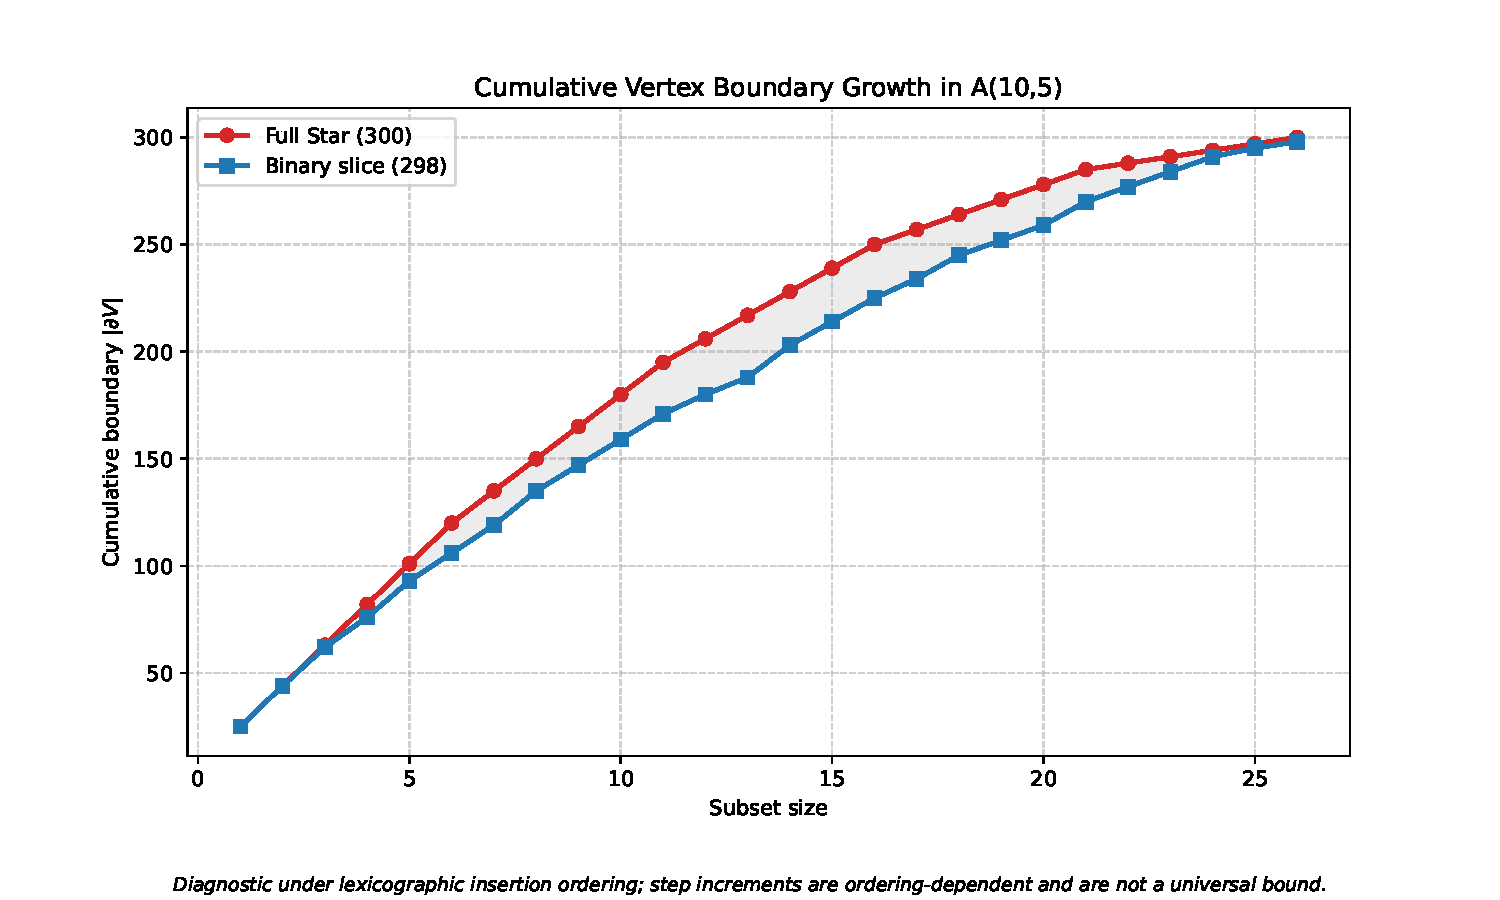
\includegraphics[width=0.9\textwidth]{../assets/out/boundary_diagnostic_plot.pdf}
	\caption{Cumulative external-boundary growth at $A(10,5)$ under
	lexicographic insertion.  The step-wise increments are path-dependent and
	serve as a diagnostic only; the terminal values ($\StarBoundary{}$ versus
	$\SliceBoundary{}$) are the insertion-order-independent boundaries of the
	two induced subgraphs.}
	\label{fig:trace}
\end{figure}

\subsection{CP-SAT certification}\label{subsec:cert}

The crossover supplies an upper bound; a lower bound requires an exhaustive
certificate.  Appendix~\ref{app:computational} gives the Boolean encoding:
binary variables $x_v, y_v$ per vertex, the volume constraint, and the boundary
implication, solved with the OR-Tools CP-SAT engine under an explicit symmetry
pin.  Because $A(10,5)$ is vertex-transitive, fixing one vertex in the subset
loses no minimum --- every $26$-subset is automorphic to one containing the
pinned vertex, and boundary size is invariant under automorphisms --- so the
certified floor is \emph{global}:
\[
	|\extbd(S)| \ge \CertFloor{} \quad\text{for every } S \text{ with } |S| = 26,
\]
and the true optimum is bracketed as
\[
	\CertFloor{} \le \min_{|S| = 26} |\extbd(S)| \le \SliceBoundary{}.
\]
We do not claim more: the search cutoff of $\HuntTarget{}$ (one below the
slice) has so far produced no feasible witness, so $\HuntTarget{}$ remains a
search target rather than a certified upper bound.


% ════════════════════════════════════════════════════════════════════════
\section{Conclusion}

This paper's contribution divides cleanly into what is proved outright and what
remains conditional, and the two should not be conflated.

\textbf{Proved unconditionally.} The Algebraic Defect Framework itself ---
the root/fiber decomposition of the external boundary into a term linear in
$(n-k)$ minus a topology-dependent correction (Section~\ref{sec:defect}), and
the subadditivity lemma underlying it --- is established outright and
mechanized in Lean~4, independent of either open proposition below. On top of
it, the Fixed-Topology Asymptotic Penalty (Theorem~\ref{thm:penalty}) is an
unconditional theorem: for every fixed sub-optimal topology, the Hamming ball's
boundary advantage grows without bound as $n-k \to \infty$, which Cheng,
Lipt\'ak, and Tian's exhaustive small-case computations
\cite{cheng2022extraconnectivity} did not establish in general. The partial
defect-spectrum classification of Section~\ref{sec:fracture} (the Topological
Funnel, its primary and secondary fractures, and Theorem~\ref{thm:classification})
is likewise proved on paper from Harper's edge-isoperimetric theorem, not
merely observed computationally.

\textbf{Conditional.} Combining these unconditional results into a single
exact closed-form boundary formula valid within the hypercube embedding
regime ($R \le 2^m$) requires the Restricted Boundary Inequality
(Proposition~\ref{prop:restricted_lower_bound}), which holds for $m \le 4$ by
computational verification but remains open for general $m$.
A second, independent
gap --- the
boundary-to-extraconnectivity reduction relating minimum-boundary sets to
exact $(R{-}1)$-extraconnectivity --- is likewise open and is not addressed by
the Lean formalization, whose capstone theorem is confined to external-neighbor
sets of $R$-element subsets.

\textbf{Net assessment.} Relative to \cite{cheng2022extraconnectivity}'s exact
computation of small-$g$ extraconnectivity cases ($g \le 6$), this paper
establishes a conditional closed-form framework that subsumes those results
within the embeddable regime. For $m \le 4$ (covering all of the paper's
canonical examples), the framework is computationally verified. Closing the
Restricted Boundary Inequality for general $m$, and the
boundary-to-extraconnectivity reduction, remain the principal open problems.

\paragraph{Conjugate geometry and local induction.}
The computational diagnostics expose a persistent trade-off between the
root-incidence defect $D(V)$ and the cross-collision multiplicity
$\sum_{w:\,\mu_V(w)\ge2}\mu_V(w)$. Sparse Star configurations have small
defect and large collision capacity, while dense Hamming-ball configurations
have the opposite profile. These quantities therefore cannot be maximized
independently in a valid extremal argument. The exact coordinate-averaged
squeeze nevertheless fails on the full Star $S_4\subset A(8,4)$: its child
potential sum is $460$, its geometric penalty is $224$, and the arithmetic
budget is $4P(17)=676$, giving the exact deficit $684-676=8$. This records a
failure of a strictly local payment rule, not a proof of a replacement
theorem; the remaining boundary problem requires a coupled argument or a
different extremal description.


% ════════════════════════════════════════════════════════════════════════
\appendix
\section{Computational Bounds and Visualizations}\label{app:computational}

Exhaustive enumeration of connected subgraphs becomes intractable beyond $R=7$.
Figure~\ref{fig:complexity} illustrates the efficiency of our $O(R^3 \log R)$
characterization engine compared to brute-force search (which grows as
$\Omega(R^{R-2})$), enabling exact boundary computation for arbitrary $R$.

\begin{figure}[H]
	\centering
	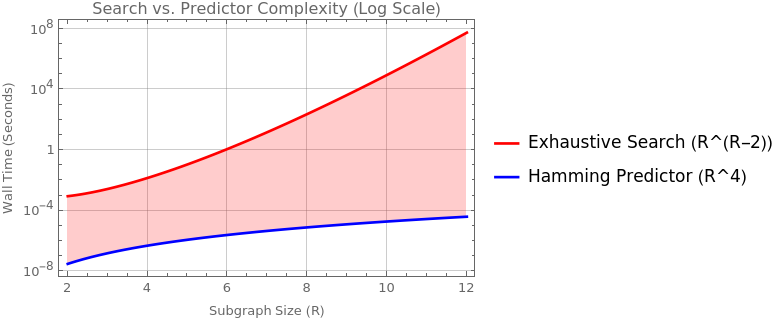
\includegraphics[width=0.8\textwidth]{../docs/complexity-curves.pdf}
	\caption{The combinatorial growth of state-space search versus our
	$O(R^3 \log R)$ engine mapping limits up to and beyond $R=128$.}
	\label{fig:complexity}
\end{figure}

Figures~\ref{fig:r9} and~\ref{fig:r10} show the induced subgraph structure of
$\mathrm{HB}_R$ for $R = 9$ and $R = 10$. Because the Hamming Ball is defined by
binary strings, this structure is independent of the host graph $A(n,k)$
(provided $n-k \ge 4$ and $k \ge 4$). Both extend the perfect $Q_3$ cube ($R=8$)
by adding vertices that share the maximum number of roots with the existing
ball.

\begin{figure}[H]
	\centering
	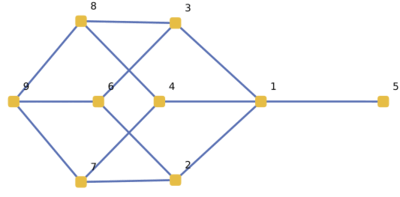
\includegraphics[width=0.5\textwidth]{../assets/out/R9_graph.png}
	\caption{Induced subgraph of $\mathrm{HB}_9$: the $Q_3$ cube plus one
	vertex, yielding $D = 13$. Valid for any $A(n,k)$ with $n-k \ge 4$,
	$k \ge 4$.}
	\label{fig:r9}
\end{figure}

\begin{figure}[H]
	\centering
	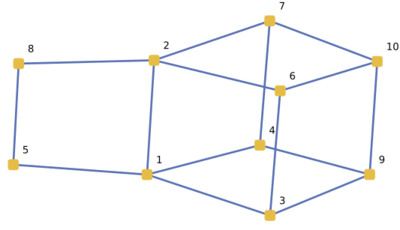
\includegraphics[width=0.5\textwidth]{../assets/out/R10_graph.png}
	\caption{Induced subgraph of $\mathrm{HB}_{10}$: the $Q_3$ cube plus two
	vertices, yielding $D = 15$. Valid for any $A(n,k)$ with $n-k \ge 4$,
	$k \ge 4$.}
	\label{fig:r10}
\end{figure}

\begin{table}[H]
	\centering
	\caption{Exact minimum-cut bounds ($R=2$ to $R=130$)}
	\small
	\begin{tabular}{ccc|ccc|ccc}
		\toprule
		$R$ & $\Eseq(R)$ & $\Cconst(R)$ & $R$ & $\Eseq(R)$ & $\Cconst(R)$ & $R$ & $\Eseq(R)$ & $\Cconst(R)$ \\
		\midrule
		2   & 1          & 1            & 45  & 115        & 136          & 88  & 268        & 308          \\
		3   & 2          & 3            & 46  & 119        & 139          & 89  & 271        & 313          \\
		4   & 4          & 4            & 47  & 123        & 142          & 90  & 275        & 317          \\
		5   & 5          & 7            & 48  & 128        & 144          & 91  & 279        & 321          \\
		6   & 7          & 9            & 49  & 130        & 149          & 92  & 284        & 324          \\
		7   & 9          & 11           & 50  & 133        & 153          & 93  & 288        & 328          \\
		8   & 12         & 12           & 51  & 136        & 157          & 94  & 293        & 331          \\
		9   & 13         & 16           & 52  & 140        & 160          & 95  & 298        & 334          \\
		10  & 15         & 19           & 53  & 143        & 164          & 96  & 304        & 336          \\
		11  & 17         & 22           & 54  & 147        & 167          & 97  & 306        & 342          \\
		12  & 20         & 24           & 55  & 151        & 170          & 98  & 309        & 347          \\
		13  & 22         & 27           & 56  & 156        & 172          & 99  & 312        & 352          \\
		14  & 25         & 29           & 57  & 159        & 176          & 100 & 316        & 356          \\
		15  & 28         & 31           & 58  & 163        & 179          & 101 & 319        & 361          \\
		16  & 32         & 32           & 59  & 167        & 182          & 102 & 323        & 365          \\
		17  & 33         & 37           & 60  & 172        & 184          & 103 & 327        & 369          \\
		18  & 35         & 41           & 61  & 176        & 187          & 104 & 332        & 372          \\
		19  & 37         & 45           & 62  & 181        & 189          & 105 & 335        & 377          \\
		20  & 40         & 48           & 63  & 186        & 191          & 106 & 339        & 381          \\
		21  & 42         & 52           & 64  & 192        & 192          & 107 & 343        & 385          \\
		22  & 45         & 55           & 65  & 193        & 199          & 108 & 348        & 388          \\
		23  & 48         & 58           & 66  & 195        & 205          & 109 & 352        & 392          \\
		24  & 52         & 60           & 67  & 197        & 211          & 110 & 357        & 395          \\
		25  & 54         & 64           & 68  & 200        & 216          & 111 & 362        & 398          \\
		26  & 57         & 67           & 69  & 202        & 222          & 112 & 368        & 400          \\
		27  & 60         & 70           & 70  & 205        & 227          & 113 & 371        & 405          \\
		28  & 64         & 72           & 71  & 208        & 232          & 114 & 375        & 409          \\
		29  & 67         & 75           & 72  & 212        & 236          & 115 & 379        & 413          \\
		30  & 71         & 77           & 73  & 214        & 242          & 116 & 384        & 416          \\
		31  & 75         & 79           & 74  & 217        & 247          & 117 & 388        & 420          \\
		32  & 80         & 80           & 75  & 220        & 252          & 118 & 393        & 423          \\
		33  & 81         & 86           & 76  & 224        & 256          & 119 & 398        & 426          \\
		34  & 83         & 91           & 77  & 227        & 261          & 120 & 404        & 428          \\
		35  & 85         & 96           & 78  & 231        & 265          & 121 & 408        & 432          \\
		36  & 88         & 100          & 79  & 235        & 269          & 122 & 413        & 435          \\
		37  & 90         & 105          & 80  & 240        & 272          & 123 & 418        & 438          \\
		38  & 93         & 109          & 81  & 242        & 278          & 124 & 424        & 440          \\
		39  & 96         & 113          & 82  & 245        & 283          & 125 & 429        & 443          \\
		40  & 100        & 116          & 83  & 248        & 288          & 126 & 435        & 445          \\
		41  & 102        & 121          & 84  & 252        & 292          & 127 & 441        & 447          \\
		42  & 105        & 125          & 85  & 255        & 297          & 128 & 448        & 448          \\
		43  & 108        & 129          & 86  & 259        & 301          & 129 & 449        & 456          \\
		44  & 112        & 132          & 87  & 263        & 305          & 130 & 451        & 463          \\
		\bottomrule
	\end{tabular}
\end{table}

\subsection{CP-SAT diagnostic searches}

In addition to exhaustive enumeration, the repository contains bounded
CP-SAT models intended as adversarial diagnostics, not as substitutes for a
universal proof.  The single-fiber model optimizes the exact collision and
defect quantities and can fix a defect shortfall.  It also reports the
proposition-equivalent residual
\[X-\bigl(\Cconst(R)-\Eseq(R)\bigr)-(m+1)\bigl(\Eseq(R)-D\bigr).
\]
The tripartite model optimizes the third-order boundary interface used in
Lemma~\ref{lem:interface-subadditivity}.  A coordinate-local model maximizes
the empty-slice residual described in Appendix~\ref{app:alt-strategies}.

For all such searches, an \texttt{OPTIMAL} status certifies the stated optimum
only for that finite $(n,k,R)$ instance; a \texttt{FEASIBLE} status is merely
an incumbent under the selected time limit.  The certified frontiers and their
witnesses are maintained in the accompanying research log.  They provide
counterexample hunting and structural examples, but do not verify
Proposition~\ref{prop:restricted_lower_bound} for arbitrary parameters.

\subsection{Exact Boolean model and certified floor}

For $A(10,5)$ the vertex set $V$ has $|V| = 30{,}240$ injective $5$-tuples.  The
model \texttt{a10\_5\_hunt} introduces per-vertex indicators: $x_v \in \{0,1\}$
with $x_v = 1$ iff $v \in S$, and $y_v \in \{0,1\}$ recording membership of $v$
in the external boundary set (exact under minimization).  The constraints
encode the set-theoretic definition of $\extbd$:
\begin{align}
	\sum_{v \in V} x_v &= 26, \label{eq:volume} \\
	x_v + y_v &\le 1 && \text{for all } v \in V, \label{eq:excl} \\
	y_v &\ge x_u - x_v && \text{for all } \{u,v\} \in E. \label{eq:bound-indicator}
\end{align}
For a fixed $x$, minimizing $\sum_v y_v$ drives $y_v$ to $0$ on selected
vertices and to $1$ exactly on external neighbors, so \eqref{eq:bound-indicator}
enforces $y_v = 1$ iff $v \in \extbd(S)$.  The model searches for subsets with
$\sum_v y_v \le \HuntTarget{}$ --- one below the $\SliceBoundary{}$-sized slice
witness --- under an imposed cutoff, and proves infeasibility iteratively.

\textbf{Global floor via a symmetry pin.}  A single vertex is pinned into $S$.
Since $A(10,5)$ is vertex-transitive, every $26$-subset is automorphic to one
containing the pinned vertex, and automorphisms preserve boundary size: a
certified floor on the pinned search is a certified floor over all subsets.
Core-guided conflict analysis has so far excluded every boundary size below
$\CertFloor{}$, and no feasible witness at or below $\HuntTarget{}$ has been
found (best = inf); the run archives more than $1.2$ million learned clauses,
each a localized geometric dead-end of $A(10,5)$.  The certified containment is
therefore
\[
	\CertFloor{} \le \min_{\substack{S \subseteq V\\ |S| = 26}} |\extbd(S)|
	\le \SliceBoundary{},
\]
with $\HuntTarget{}$ a search target rather than an upper bound.  This floor is
an evolving lower-bound record --- each successive core raises it --- and is
tracked in the accompanying research log.

\begin{remark}[Coordinate-edge counting]\label{rem:coord-edges}
Let $\CoordEdges(S)$ denote the total number of coordinate-aligned edges from
members of $S$ to the external boundary, counted per source coordinate:
$\CoordEdges(S) = \sum_{p=1}^{k} |\partial_p(S)|$, where $\partial_p(S)$ is the
set of external neighbors that differ from $S$ in position $p$.  Two exact
identities determine it from the defect-framework data alone:
\begin{equation}\label{eq:coord-edges}
	\CoordEdges(S) = |\extbd(S)| + X(S) = U(S)\,(m+1) - |S|\,k,
\end{equation}
where $U(S) = \sum_p |U_p(S)|$ is the total unique-root count
(eq.~\eqref{eq:unique-roots}), $m = n-k$, and
$X(S) = \CoordEdges(S) - |\extbd(S)|$ is the cross-collision surplus of
Section~\ref{sec:defect}: the excess of per-coordinate boundary incidences over
distinct boundary vertices.  The second equality counts, per occupied root
$r \in U(S)$, the $(m+1)$ vertices on its line minus those already selected
into $S$; every such external vertex is adjacent to all members on that line.
For the $26$-subsets of the bracket above, this ties the boundary size to a
single geometric count --- equivalently to the occupied-root count, since
$D(S) = k|S| - U(S)$.
\end{remark}


% ════════════════════════════════════════════════════════════════════════
\section{Formal verification in Lean 4}\label{app:lean}

The Lean development mechanizes the coordinate-root boundary identity, the
defect inequality, the ordered Bonferroni overlap estimate, the global
witness-pair charging bound, and the resulting additive-error boundary
estimate. The Hamming-ball collision count is proved directly, giving an
exact evaluation of that construction. These components compose in the
capstone module to prove the boundary-profile sandwich and the first-order
profile estimate. The public theorem states a boundary-profile sandwich, not
exact optimality and not an extra-connectivity formula.

The source modules implement root counts, boundary decomposition, collision
charging, Hamming-ball evaluation, and the profile capstone. The theorem audit
checks the active capstone dependency terms for \texttt{sorryAx}. Refuted
exact-boundary statements and their
finite counterexample certificates are kept outside this active dependency
chain. The general Star-cut connectivity theorem, a classification of
intermediate extremizers, and the reduction from the boundary profile to
$\kappa_g$ are not formalized here.

In the Lean source, \texttt{E\_seq} and \texttt{C\_constant} represent
$E(R)$ and $C(R)$, respectively. The additive error in the formal theorem is
$E(R)+2(R^2-R)$.


% ════════════════════════════════════════════════════════════════════════
\section{Characterization Engine Source Code}\label{app:engine}

The $O(R^3 \log R)$ characterization engine that computes exact boundary
formulas for arbitrary $R$ is listed below (C++17). The engine operates in three
tiers: (1)~analytical evaluation of $\Eseq(R)$ and $\Cconst(R)$ in $O(R)$ time,
(2)~constructive Hamming Ball computation and formula verification in $O(R^3)$
time, and (3)~brute-force neighbor enumeration in $O(R^3 \log R)$ time. The full
source repository is available at
\href{https://github.com/ou-school-repos/program-arrangement-extraconnectivity}{\texttt{github.com/ou-school-repos/program-arrangement-extraconnectivity}}
and an excerpt is provided below (\texttt{predict.cpp}).

\paragraph{Implementation details.}
The engine is designed for exact integer arithmetic. Vertex representations use
an inline fixed-capacity array (\texttt{Vertex<K,SymT>}) templatized on both a
compile-time capacity $K$ and the symbol type: \texttt{uint8\_t} for $R \le 127$
and \texttt{uint16\_t} for $128 \le R \le 260$. The verification tiers choose
$K$ close to the actual $R$, reducing the constant factor in the $\Theta(R^3
\cdot K)=\Theta(R^4)$ peak storage used for brute-force neighbor enumeration.
Sorting and deduplication use the lexicographical comparison operators of
\texttt{std::array}. The final boundary computation is promoted to
\texttt{\_\_int128}, while the inner loops use native integer arithmetic.

\embedfile[filespec=predict.cpp,desc={Characterization engine source (C++17)}]{../src/predict.cpp}

\lstinputlisting[language=C++]{predict_core_sample.cpp}

\noindent \emph{Note:} In the C++ source, the struct fields \texttt{nk1} and
\texttt{constant} correspond to $\Eseq(R)$ and $\Cconst(R)$ respectively. This
engine checks Proposition~\ref{prop:hb-eval} by verifying \\
\texttt{brute\_force\_neighbors(verts, 2 * R, R) == (R * R - nk1) * R -
constant} \\ for all $R \le 160$, giving strong numerical evidence that the
Hamming Ball achieves the exact boundary predicted by Theorem~\ref{thm:main}.
Because the Algebraic Defect Framework decouples the network dimensions from the
subset structure, this paper leverages a property of $A(n,k)$, that the
constants $\Eseq(R)$ and $\Cconst(R)$ are strictly independent of $n$ and $k$;
thus, verifying the boundary for the dense embedding $n=2R$, $k=R$ is sufficient
to guarantee the formula's exactness for all valid dimensions.
Proposition~\ref{prop:universal} quantifies over \emph{all} subsets, whereas
the \texttt{nauty}-based search tests connected $R$-vertex subsets for
$R \le 10$; it is therefore partial evidence rather than a verification of the
universal proposition.


% ════════════════════════════════════════════════════════════════════════
\section{Future ideas for Proving the Universal Boundary Inequality}\label{app:alt-strategies}

\begin{quote}
\textit{Everything in this appendix is a research sketch, not a result.
Nothing here is proven, checked, or claimed to be correct; it is recorded
only so that future work on Proposition~\ref{prop:universal} does not
restart from nothing. Neither strategy below has been carried past an
informal whiteboard stage.}
\end{quote}

The coordinate-root compression approach outlined in the accompanying
research notes (\texttt{docs/proof-\allowbreak sketch-\allowbreak weighted-potential.md}) stalls
on a coordinate-tangling obstacle: a local compression move at position
$p$ unavoidably scrambles roots at every other position $q \neq p$, and no
argument to date bounds that scatter damage tightly enough to recover
monotonicity of $X(V') + (m+1)D(V')$. Three alternative directions are
sketched below.

\paragraph{Marginal induction with partial-layer tracking.}
This direction extends the proof skeleton already used for
Theorem~\ref{thm:defect} (proven by strong induction on $R$, partitioning
$V'$ by a coordinate and applying Lemma~\ref{lem:subadditivity}), carrying
the joint quantity $\Phi = X + (m+1)D$ instead of $D$ alone. Stripping a
vertex $v$ with $s$ roots shared with the remaining $R-1$ vertices gives
$\Delta D = s$ exactly; closing the induction would require bounding
$\Delta X$ as a function of $s$ and $m$ alone, so that
$\Delta X + (m+1)s \le \Delta \Cconst(R) + m \cdot \Delta \Eseq(R)$. A
partial result toward this bound has since been derived (not yet
mechanized in Lean): writing out the marginal change in
$\mathrm{total\_coord\_edges}$ gives $\Delta X \le (k-s)m$ unconditionally,
and separately $\Delta X = 0$ whenever $v$ is adjacent to the vertex
removed (proved directly from the one-coordinate-difference property of
adjacency, independent of $n,k,R$). A second, dimension-independent cap
$\Delta X \le 2(R-1)$ also holds, from the fact that only vertices at
Hamming distance $2$ from $v$ can contribute to $\Delta X$ via a fresh
root. Whether $\min\big((k-s)m,\,2(R-1)\big)$ always suffices to close the
induction is conjectured but unproved; only two supporting configurations
have been checked (see \texttt{docs/proof-sketch-weighted-potential.md}
for the derivations and the open reconciliation with $\Delta \Cconst(R)$).

\paragraph{Dual root-compression via averaging.}
Inspired by Pinto's resolution of the Bollob\'{a}s--Leader directed-path
conjectures on the hypercube \cite{pinto2015directed}, where two
compression operators that each individually fail to shrink a directed
boundary are shown to satisfy an averaging inequality forcing at least
one of them to be non-worsening. The single guarded-symbol compression
already refuted on $A(n,k)$ (Section~\ref{sec:nogo}) is one such
individually-failing operator; whether a dual pair of root-compression
operators exists on $A(n,k)$, respecting the injectivity constraint, for
which an analogous averaging bound holds for $X+(m+1)D$, is entirely
untried. This is flagged only as a structural analogy worth investigating
for the coordinate-tangling obstacle; no candidate operator pair has been
proposed.

\paragraph{A global Lyapunov function on fiber multisets.}
This direction proposes a potential $\Phi(V') = \sum_{p=1}^k \sum_r
f(|F_{p,r}|)$ over the multiset of fiber sizes at every coordinate, for
some convex $f$, and asks whether a single root-compression move's local
gain (from concentrating vertices into larger fibers at one coordinate)
always dominates its collateral loss (from scrambling roots at every other
coordinate). Neither the link between this $\Phi$ and $X + (m+1)D$, nor
the required domination bound, has been established; it is not known
whether a suitable $f$ exists.

\medskip
\noindent Of the three, the marginal-induction direction is judged most
advanced in practice, since its early steps reuse machinery already
mechanized in Lean (Lemma~\ref{lem:subadditivity} and
Theorem~\ref{thm:defect}'s induction) and its open step now has a partial
derivation rather than being untouched. The dual-compression direction is
flagged as a promising untried structural analogy, precisely because it
targets the coordinate-tangling obstacle that stalled the original
single-operator compression, but nothing on $A(n,k)$ has been attempted
for it yet. The Lyapunov direction remains a from-scratch invariant
search with no candidate potential shown to work. These are research
opinions, not mathematical claims, and should not be read as evidence
toward Proposition~\ref{prop:universal} itself.


\bibliographystyle{plain}
% \nocite{*}
\bibliography{references}

\end{document}
